\subsection{Further learnings}
\label{subsec:dlu}

The two official problems of this section treat a supervised MLP pipeline and a continuous-time VP diffusion. The official syllabus, and the later papers, ask for several neighbouring objects that Problem~2's scope list already named. The notes below collect those objects in the same format as the Machine Learning further-learnings block: a definition or proposition, a remark that ties the object back to Problem~1 or Problem~2, and an exercise with a fully written solution. Reinforcement learning is \emph{not} rewritten here; it already occupies \jump{sec:rl-supplement}{the RL supplement}. Self-attention at NLP length already occupies Part~D; this block keeps only the deep-learning exam formulas (parameter counts, scaling, a minimal vision transformer).


\subsubsection{Backpropagation, activations, and momentum}
\label{subsubsec:dlu-backprop}

Problem~1 already uses backpropagation as the algorithm that produces the mini-batch gradient \(g_t\), and already writes momentum and Adam as rules that \emph{consume} \(g_t\). Later papers ask for the chain-rule formula itself, for the cost comparison with a forward pass, and for the vanishing-gradient contrast between sigmoid and ReLU.

\begin{notation}[Layerwise network]
\label{not:dlu-mlp}
Write a feedforward net as
\[
x_\ell = f_\ell(x_{\ell-1},\theta_\ell),
\qquad
\ell=1,\dots,L,
\]
with input \(x_0=x\) and scalar loss \(\mathcal{J}=\mathcal{L}(x_L,y)\). Here \(\theta_\ell\) are the parameters of layer \(\ell\) only (weights and bias of that layer).
\end{notation}

\begin{proposition}[Layerwise gradient]
\label{prop:dlu-layer-grad}
By the chain rule,
\[
\frac{\partial\mathcal{J}}{\partial\theta_\ell}
=
\frac{\partial\mathcal{J}}{\partial x_\ell}\,
\frac{\partial x_\ell}{\partial\theta_\ell},
\qquad
\frac{\partial\mathcal{J}}{\partial x_{\ell-1}}
=
\frac{\partial\mathcal{J}}{\partial x_\ell}\,
\frac{\partial x_\ell}{\partial x_{\ell-1}}.
\]
The second identity is the backward recurrence: once \(\partial\mathcal{J}/\partial x_\ell\) is known, the error signal at the previous layer is a Jacobian--vector product against the layer map \(f_\ell\).
\end{proposition}

\begin{remark}[Same order as one forward evaluation]
\label{rem:dlu-reverse-mode}
A forward evaluation computes every \(x_\ell\) and \(\mathcal{J}\) once. Reverse-mode automatic differentiation then sends a scalar error signal backward, performing one Jacobian--vector product per layer. The arithmetic is a small constant times the forward cost, independently of \(\dim\theta\). Forward-mode differentiation, by contrast, would cost a factor \(\dim\theta\). This is why Problem~1 can treat \(g_t=\nabla_\theta J(\theta_t)\) as a computable object rather than an oracle.
\end{remark}

\begin{proposition}[Sigmoid saturation versus ReLU]
\label{prop:dlu-vanish}
Let \(\sigma(z)=(1+e^{-z})^{-1}\). Then \(\sigma'(z)=\sigma(z)(1-\sigma(z))\le 1/4\), with equality only at \(z=0\). In a deep stack the backward signal is multiplied by a product of such factors and of weight matrices; if the pre-activations leave a neighbourhood of \(0\), the product collapses and \(\partial\mathcal{J}/\partial\theta_1\) vanishes. ReLU\((z)=\max\{0,z\}\) has derivative \(1\) on \(\{z>0\}\), so a path of active units transmits the error without a \(1/4\) factor at every layer. Dead ReLUs (\(z<0\) throughout training) are a different failure mode, not a cure-all.
\end{proposition}

\begin{exercise}[Write the two chain-rule factors]
\label{ex:dlu-chain}
Consider a two-layer map \(x_1=\sigma(W_1 x_0+b_1)\), \(x_2=W_2 x_1+b_2\), and \(\mathcal{J}=\frac12\|x_2-y\|^2\). Write \(\partial\mathcal{J}/\partial W_1\) by naming every intermediate Jacobian. Then explain in one paragraph why computing both \(\partial\mathcal{J}/\partial W_1\) and \(\partial\mathcal{J}/\partial W_2\) is the same order as evaluating \(\mathcal{J}\).
\end{exercise}

\begin{solution}[Write the two chain-rule factors]
\textbf{Step 1: name the forward objects.}
Let \(a_1=W_1 x_0+b_1\) and \(x_1=\sigma(a_1)\) (componentwise). The loss depends on \(W_1\) only through \(a_1\to x_1\to x_2\).

\textbf{Step 2: the last layer is elementary.}
\[
\frac{\partial\mathcal{J}}{\partial x_2}=x_2-y,
\qquad
\frac{\partial\mathcal{J}}{\partial W_2}
=
(x_2-y)\,x_1^\top.
\]
(If one prefers index notation: \(\partial\mathcal{J}/\partial (W_2)_{jk}=(x_2-y)_j\,(x_1)_k\).)

\textbf{Step 3: send the error to layer 1.}
\[
\frac{\partial\mathcal{J}}{\partial x_1}
=
W_2^\top(x_2-y),
\qquad
\frac{\partial\mathcal{J}}{\partial a_1}
=
\bigl(W_2^\top(x_2-y)\bigr)\odot\sigma'(a_1),
\qquad
\frac{\partial\mathcal{J}}{\partial W_1}
=
\frac{\partial\mathcal{J}}{\partial a_1}\,x_0^\top.
\]
The three displayed factors are exactly \(\partial\mathcal{J}/\partial x_\ell\), \(\partial x_\ell/\partial a_\ell\), and \(\partial a_\ell/\partial W_\ell\) in \cref{prop:dlu-layer-grad}.

\textbf{Step 4: cost.}
The forward pass already multiplies by \(W_1\) and \(W_2\) and evaluates \(\sigma\). The backward pass multiplies by \(W_2^\top\), by the diagonal \(\sigma'(a_1)\), and by \(x_0^\top\). Each of those products has the same leading dimension as the corresponding forward product. No extra loop over the coordinates of \(W_1\) is required: reverse mode reuses the cached \(x_0,a_1,x_1\). That is the ``same order as one forward evaluation'' claim of Spring 2026 Problem~1(a)(ii).
\end{solution}

\begin{exercise}[Why sigmoid vanishes and ReLU need not]
\label{ex:dlu-relu}
Let \(z\in\mathbb{R}\) and suppose a backward factor \(\delta\) arrives at a neuron. Compare \(\lvert\delta\cdot\sigma'(z)\rvert\) with \(\lvert\delta\cdot\mathrm{ReLU}'(z)\rvert\) in the two regimes \(z=0\) and \(z=4\). What does this imply for a product of twenty such factors?
\end{exercise}

\begin{solution}[Why sigmoid vanishes and ReLU need not]
At \(z=0\), \(\sigma'(0)=1/4\) and \(\mathrm{ReLU}'(0)\) may be defined as \(0\) or \(1\) by convention; the exam contrast is not at the kink. At \(z=4\),
\[
\sigma(4)=\frac{1}{1+e^{-4}}\approx 0.982,
\qquad
\sigma'(4)\approx 0.018,
\]
while \(\mathrm{ReLU}'(4)=1\). A single saturated sigmoid already multiplies the error by about \(1/50\). Twenty independent factors of size \(1/4\) (the most favourable sigmoid bound) give \(4^{-20}<10^{-12}\). Twenty ReLU factors along an active path give \(1\). Hence deep sigmoid stacks silently stop training the early layers, which is the vanishing-gradient problem named in Spring 2026 Problem~1(b). ReLU removes that systematic contraction; it does not remove the need for a sensible initialization, nor the dead-unit issue on the negative half-line.
\end{solution}

\begin{proposition}[SGD with momentum, exam form]
\label{prop:dlu-mom}
Let \(g_k\) be the mini-batch gradient at the current parameter \(x_k\), and fix \(\beta\in[0,1)\) and \(\eta>0\). The classical heavy-ball updates are
\[
v_{k+1}
=
\beta v_k+g_k,
\qquad
x_{k+1}
=
x_k-\eta v_{k+1},
\]
with \(v_0=0\). This is the same pair already written in Problem~1 as \(v_{t+1}=\beta v_t+g_t\), \(\theta_{t+1}=\theta_t-\eta_t v_{t+1}\). Compared with plain SGD \(x_{k+1}=x_k-\eta g_k\), a consistent direction accumulates in \(v\), while an oscillating coordinate is partially cancelled. Adam is not rewritten here: it is the first-moment-plus-second-moment-plus-bias-correction rule already recorded in Problem~1.
\end{proposition}

\begin{exercise}[Write the two momentum lines]
\label{ex:dlu-mom}
Write \(v_{k+1}\) and \(x_{k+1}\) for SGD with momentum. In one sentence, say what happens to \(v\) when consecutive \(g_k\) have opposite signs on a coordinate.
\end{exercise}

\begin{solution}[Write the two momentum lines]
\[
v_{k+1}=\beta v_k+g_k,
\qquad
x_{k+1}=x_k-\eta v_{k+1},
\]
with \(v_0=0\) and \(\beta\in[0,1)\) (typically near \(0.9\)). Opposite signs on a coordinate make the new \(g_k\) cancel part of the stored \(v_k\), so the step along that axis shrinks. That is the oscillation-damping claim of Spring 2026 Problem~1(c). Persistent signs do the opposite: \(v\) grows and the step is larger than a single \(g_k\).
\end{solution}


\subsubsection{Convolutions, attention, and a minimal vision transformer}
\label{subsubsec:dlu-cnn-attn}

Problem~1 never counts convolutional parameters and never writes \(Q,K,V\). Fall 2025 Problem~1 and Spring 2026 Problem~1(d)--(e) do. The long conceptual discussion of self-attention lives in Part~D; the identities below are the deep-learning exam layer.

\begin{proposition}[Convolutional parameter count]
\label{prop:dlu-cnn-params}
A 2D convolutional layer with kernel size \(k\times k\), \(C_{\mathrm{in}}\) input channels, \(C_{\mathrm{out}}\) output channels, and a bias per output channel has
\[
C_{\mathrm{out}}\bigl(k^{2}C_{\mathrm{in}}+1\bigr)
\]
trainable scalars. A dense layer mapping the same flattened input \(H\times W\times C_{\mathrm{in}}\) to an output of shape \(H'\times W'\times C_{\mathrm{out}}\) has
\[
\bigl(HWC_{\mathrm{in}}\bigr)\bigl(H'W'C_{\mathrm{out}}\bigr)+H'W'C_{\mathrm{out}}
\]
parameters. Convolution is smaller because the same \(k\times k\times C_{\mathrm{in}}\) kernel is shared across spatial locations.
\end{proposition}

\begin{remark}[Why convolution helps vision]
\label{rem:dlu-cnn-inductive}
Locality and translation sharing are the inductive bias that Problem~1 already named when it recommended a CNN for images. The count in \cref{prop:dlu-cnn-params} is the quantitative form of that sentence: the hypothesis class is much smaller than the dense class of the same input--output shape, so the training-error-versus-test-error tension of Problem~1(e) is milder for a well-specified convolution than for an MLP on pixels.
\end{remark}

\begin{definition}[Scaled dot-product attention]
\label{def:dlu-sdp}
Given queries, keys, and values \(Q,K\in\mathbb{R}^{L\times d_k}\), \(V\in\mathbb{R}^{L\times d_v}\),
\[
\mathrm{Attn}(Q,K,V)
=
\mathrm{softmax}\Bigl(\frac{QK^\top}{\sqrt{d_k}}\Bigr)V.
\]
Row \(i\) of the softmax is a distribution on source positions; row \(i\) of the output is the corresponding average of the value rows. The maps \(Q=XW_Q\), \(K=XW_K\), \(V=XW_V\) are learned.
\end{definition}

\begin{proposition}[Role of \(1/\sqrt{d_k}\)]
\label{prop:dlu-scale}
If the entries of \(q,k\in\mathbb{R}^{d_k}\) are independent of variance \(1\), then \(\mathrm{Var}(\langle q,k\rangle)=d_k\). Without the scale, the softmax logits have standard deviation \(\sqrt{d_k}\) and, for large \(d_k\), concentrate on a one-hot vector. The Jacobian of softmax at a one-hot vector vanishes, so gradients die. Dividing by \(\sqrt{d_k}\) keeps the logits \(O(1)\).
\end{proposition}

\begin{remark}[Position is not in \(QK^\top\)]
\label{rem:dlu-pos}
Permutation of the \(L\) rows of \(X\) permutes the output of \cref{def:dlu-sdp} accordingly: the mechanism is equivariant and has no preferred order. Images and language are not sets. One therefore adds a positional encoding (sinusoidal, learned, or relative) to the patch or token embeddings before forming \(Q,K,V\). This is the same necessity that Part~D discusses at greater length.
\end{remark}

\begin{construction}[A minimal convolution--attention vision model]
\label{con:dlu-vit}
Tokenize an image \(H\times W\times C\) by a non-overlapping \(P\times P\) convolution (or a linear map on flattened patches) into \(N=HW/P^{2}\) patch embeddings of width \(d\). Add a positional encoding of shape \(N\times d\). Apply one or more Transformer blocks (self-attention as in \cref{def:dlu-sdp}, then a tokenwise MLP). Read a class token, or pool the \(N\) outputs, into the classifier head of Problem~1(a). Convolution may sit in the stem (the patch embedding itself) or as a local mixer inside each block. Self-attention supplies the global interactions that a small stack of \(3\times 3\) convolutions would need many layers to transport.
\end{construction}

\begin{exercise}[Design the hybrid in three places]
\label{ex:dlu-vit}
For an image \(H\times W\times C\), name: (i) how the tokens are produced; (ii) where self-attention is applied; (iii) where a convolution is introduced. Then give one sentence each for the benefit of convolution and the benefit of attention.
\end{exercise}

\begin{solution}[Design the hybrid in three places]
(i) Split the image into non-overlapping \(P\times P\) patches and map each patch to a \(d\)-vector by a linear layer or, equivalently, by a \(P\times P\) convolution of stride \(P\); add a positional encoding (and optionally a class token). (ii) Self-attention, as in \cref{def:dlu-sdp}, runs among the \(N=HW/P^{2}\) tokens inside each Transformer block. (iii) Convolution sits in the stem that produces the patch embeddings, or as a local mixer beside the attention block; naming ``ViT'' without placing the convolution is not a design.

Convolution: local translation-shared feature extraction, with the parameter count of \cref{prop:dlu-cnn-params}. Attention: content-dependent global mixing in one layer, which a small \(3\times 3\) stack cannot do. That is Fall 2025 Problem~1(c) and \cref{con:dlu-vit}.
\end{solution}

\begin{exercise}[Count the convolutional parameters]
\label{ex:dlu-cnn-count}
A layer has \(H=W=32\), \(C_{\mathrm{in}}=3\), \(k=3\), \(C_{\mathrm{out}}=16\), and a bias. Compute its number of parameters. Then compute the parameter count of a dense layer that maps the flattened \(32\times 32\times 3\) input to a \(32\times 32\times 16\) output. What ratio do you obtain, and what does the ratio measure?
\end{exercise}

\begin{solution}[Count the convolutional parameters]
Convolution:
\[
16\bigl(3^{2}\cdot 3+1\bigr)
=
16\cdot(27+1)
=
448.
\]
Dense:
\[
(32\cdot 32\cdot 3)\cdot(32\cdot 32\cdot 16)+32\cdot 32\cdot 16
=
3072\cdot 16384+16384
=
50\,347\,648.
\]
The ratio is about \(1.1\times 10^{5}\). It measures the parameter saving from sharing one \(3\times 3\times 3\) kernel across \(32^{2}\) locations, which is exactly the translation-invariance bias of \cref{rem:dlu-cnn-inductive}. Fall 2025 Problem~1(a) is this computation; omitting the \(+C_{\mathrm{out}}\) bias is the usual half-point loss.
\end{solution}

\begin{exercise}[Attention without the scale]
\label{ex:dlu-scale}
Suppose \(d_k=256\) and a query--key pair has \(\langle q,k\rangle=32\) before scaling (a typical \(O(\sqrt{d_k})\) draw). Compare the two softmax weights obtained from logits \((32,0)\) and from logits \((32/\sqrt{256},0)=(2,0)\). What happens to \(\partial\mathrm{softmax}/\partial\mathrm{logit}\) in the first case?
\end{exercise}

\begin{solution}[Attention without the scale]
Unscaled:
\[
\mathrm{softmax}(32,0)
=
\Bigl(\frac{e^{32}}{e^{32}+1},\frac{1}{e^{32}+1}\Bigr)
\approx
(1,0).
\]
Scaled:
\[
\mathrm{softmax}(2,0)
=
\Bigl(\frac{e^{2}}{e^{2}+1},\frac{1}{e^{2}+1}\Bigr)
\approx
(0.88,0.12).
\]
In the unscaled case the distribution is numerically one-hot. If \(p=\mathrm{softmax}(z)\) and \(p\approx e_1\), the Jacobian \(D\mathrm{softmax}=\mathrm{diag}(p)-pp^\top\) is approximately zero. The value vectors then receive no usable gradient through the attention weights. That is Spring 2026 Problem~1(d). The factor \(1/\sqrt{d_k}\) exists to keep the softmax in the regime where several sources still share mass.
\end{solution}

\begin{exercise}[RNN versus Transformer, in one computational-graph sentence each]
\label{ex:dlu-rnn}
Give two reasons why a Transformer is typically more efficient than an RNN on modern accelerators, and state the quadratic caveat.
\end{exercise}

\begin{solution}[RNN versus Transformer]
An RNN must evaluate \(h_t=f(h_{t-1},x_t)\) in order of \(t=1,\dots,L\); the compute graph is a path of length \(L\), so a signal from token \(1\) to token \(L\) travels \(L-1\) multiplications and the \(L\) steps cannot be batched in the time direction. A Transformer forms \(QK^\top\) as one matrix product of shape \(L\times L\); every pair \((i,j)\) interacts inside a single layer and the \(L\) query rows are independent given \(K,V\). Accelerators like large matmuls. The caveat is cost \(O(L^{2}d)\) in sequence length, which is why long-context variants exist. This is Spring 2026 Problem~1(e) and is the same comparison as Part~D's Transformer-versus-recurrent question, written from the hardware side rather than the language-modelling side.
\end{solution}


\subsubsection{Approximation and generalization for networks}
\label{subsubsec:dlu-approx}

The syllabus names ``approximation and generalization analysis'' as part of deep-learning foundations. Problem~1 treats the same tension operationally (widen the net versus regularize the net). The Machine Learning further-learnings block already records the classical VC story and a pointer to constructive universal approximation. The remarks below only record what changes when the hypothesis class is a deep net.

\begin{remark}[Approximation is not learnability]
\label{rem:dlu-ua-not-pac}
A sigmoid MLP is dense in \(C([-1,1]^n)\) (Fall 2025 Machine Learning Problem~13). Density says: some parameter realizes a small uniform error. It does not say that SGD on a finite sample finds that parameter, nor that the class of thresholded networks has finite VC dimension. Spring 2026 Machine Learning MQ3 is the corresponding warning for ReLU: piecewise-linear complexity grows with depth and width; universal approximation does not imply PAC learnability.
\end{remark}

\begin{remark}[Two regularizers, already in Problem~1]
\label{rem:dlu-two-reg}
Weight decay is an explicit penalty on \(\theta\), the same \(\tfrac{\lambda}{2}\|\theta\|^2\) that Problem~4 of Part~A analyses for stability. Dropout and early stopping are implicit: they change the algorithm \(A(S)\) without changing the nominal training loss. Overparameterized nets can interpolate \(S\) and still generalize; that phenomenon is not explained by the finite-VC theorem of Part~A, and is the ``network implicit regularization'' item of the official syllabus.
\end{remark}


\subsubsection{A dictionary of vision tasks}
\label{subsubsec:dlu-vision}

The official syllabus lists feature extraction, image restoration, three-dimensional reconstruction, optical flow, recognition, and segmentation. Problem~1 is recognition. Problem~2 briefly mentions restoration as a conditional inverse problem. The other items have not appeared as standalone deep-learning questions; they are recorded here as input--output--loss triples that reuse the extractor-plus-head template of Problem~1(a).

\begin{center}
{\footnotesize
\begin{tabularx}{\linewidth}{|p{3.1cm}|X|X|X|}
\hline
\textbf{Task} & \textbf{Input / output} & \textbf{Typical loss} & \textbf{Link to this paper} \\ \hline
Feature extraction & \(x\mapsto z=e_{\theta_F}(x)\) & none by itself; trained by a head & Problem~1(a), the MLP extractor \\ \hline
Recognition & image \(\to\Delta^{C-1}\) & softmax cross-entropy & Problem~1 \\ \hline
Segmentation & image \(\to\) per-pixel labels & per-pixel cross-entropy & same pipeline; head is spatial \\ \hline
Restoration / super-resolution & degraded \(y\to\widehat x\) & \(\|A\widehat x-y\|^2\) plus a prior & Problem~2, conditional score \(\nabla\log p_t(x\mid c)\) \\ \hline
Optical flow & pair of frames \(\to\) displacement field & photometric + smoothness, or supervised \(L^2\) & a regression head on a Siamese extractor \\ \hline
3D reconstruction & views \(\to\) depth, voxels, or an implicit field & rendering / multi-view consistency & a generative prior on geometry or appearance \\ \hline
\end{tabularx}
}
\end{center}

\begin{exercise}[Name the spaces for segmentation]
\label{ex:dlu-seg}
Rewrite Problem~1(a) for semantic segmentation of a \(C\)-class image of size \(H\times W\). What is the output space of the classifier head, and what is the natural loss?
\end{exercise}

\begin{solution}[Name the spaces for segmentation]
The extractor \(e_{\theta_F}\) may still map the image to a feature tensor, now of shape \(H'\times W'\times m\) rather than a vector in \(\mathbb{R}^m\). The classifier head maps each spatial site to \(\Delta^{C-1}\), so the network output lives in \((\Delta^{C-1})^{H\times W}\) after upsampling. The loss is the average of the Problem~1 softmax cross-entropies over the \(HW\) pixels (possibly reweighted for rare classes). Nothing in the five-piece slogan ``data \(\to\) model \(\to\) loss \(\to\) optimization \(\to\) evaluation'' has changed; only the output space is a field of distributions rather than one distribution.

\begin{center}
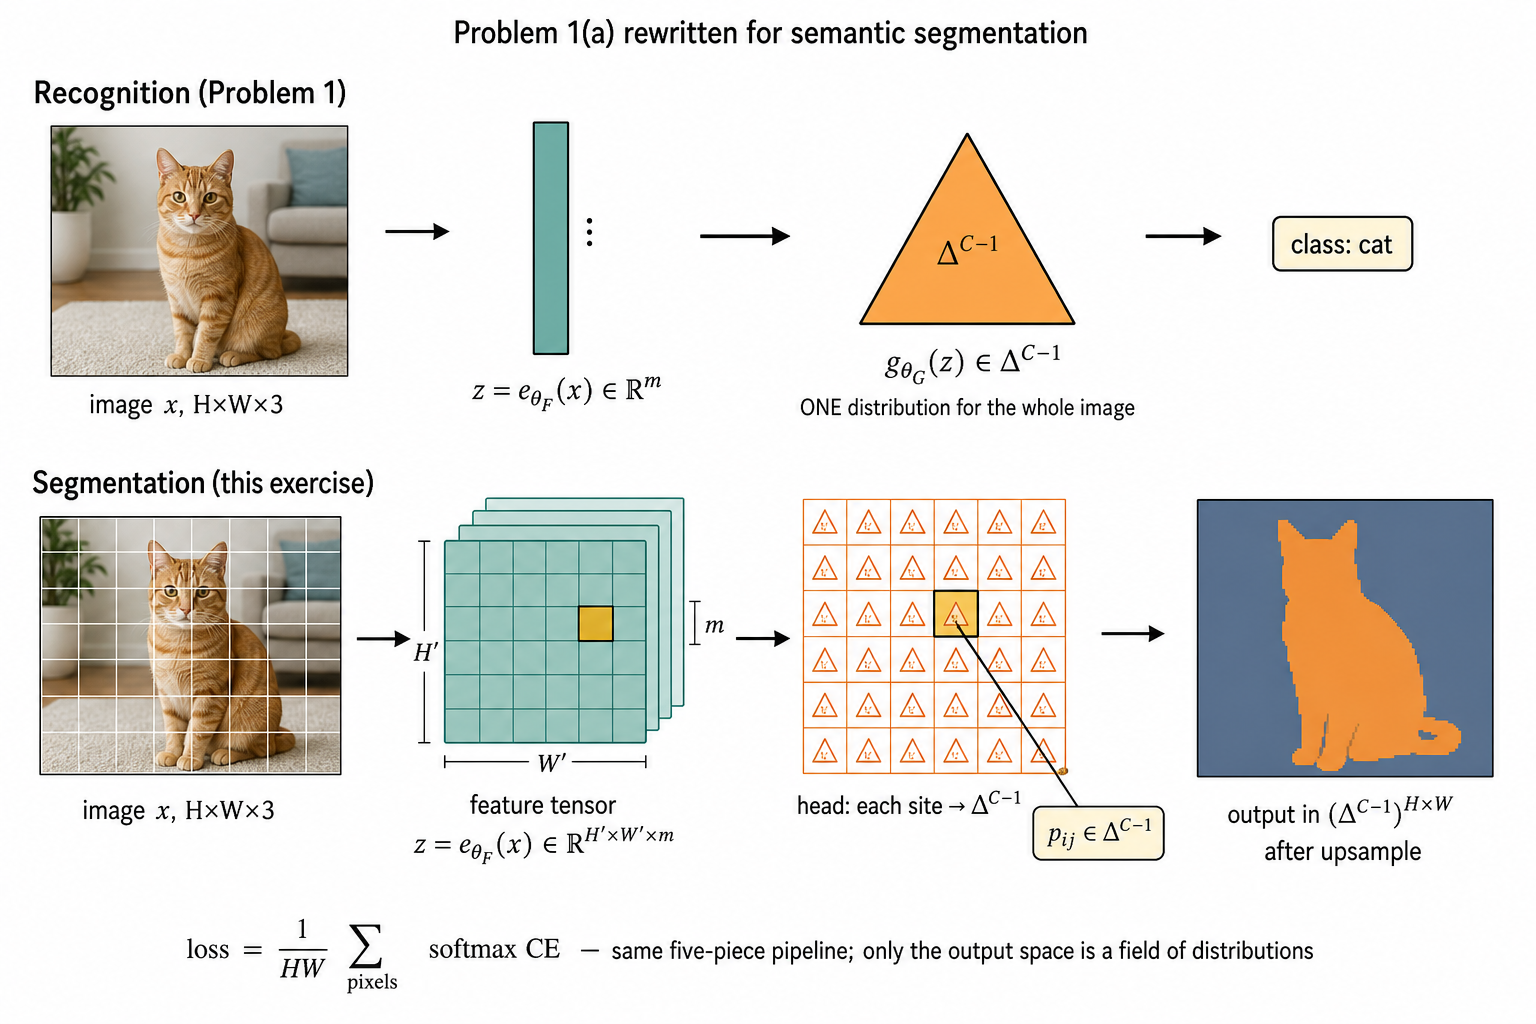
\includegraphics[width=0.96\linewidth]{figures/vision/seg-spaces-pipeline.png}\\[0.35em]
{\small Recognition keeps a single feature vector \(z\in\mathbb{R}^m\) and one simplex. Segmentation keeps a spatial feature tensor \(z\in\mathbb{R}^{H'\times W'\times m}\); the same head is applied at every site.}
\end{center}
\end{solution}


\subsubsection{Unsupervised, contrastive, transfer, and implicit regularization}
\label{subsubsec:dlu-unsup}

The title is the official syllabus bullet, not a natural mathematical partition: ``unsupervised learning: autoencoders, contrastive learning, implicit regularization of networks, transfer learning and meta-learning.'' Problem~1 is fully supervised. One already has pairs \((x_i,y_i)\) and trains \(f_\theta=g_{\theta_G}\circ e_{\theta_F}\) by softmax cross-entropy. This block answers the neighbouring question that the syllabus attached to that extractor: if the label \(y\) is missing or scarce, \emph{what scalar still trains} \(e_{\theta_F}\), and how is the resulting representation \(z=e_{\theta_F}(x)\) reused as the backbone of Problem~1(a)?

The four title words are four different answers, and they are not synonyms. An \emph{autoencoder} is classical unsupervised representation learning: reconstruct \(x\) from a bottleneck and keep the encoder. \emph{Contrastive} learning---and, more generally, self-supervised learning---still uses no human \(y\), but manufactures a surrogate label from the data itself (two augmented views of one image, a masked token, the next token) and trains \(e\) to agree on positives and disagree on negatives; InfoNCE is the exam formula. ``Self-supervised'' is the modern name for that manufacturing; the syllabus's older umbrella is ``unsupervised.'' Contrastive learning is one family inside self-supervision, not a synonym for all of it. \emph{Transfer} (and meta-learning) assume some labels exist \emph{somewhere}: pretrain \(e\) by reconstruction, by contrastive pairs, or on a large source task, then replace or retrain the head \(g\) on a small target. That is exactly the extractor--head table already written in Problem~1. \emph{Implicit regularization} is the odd item in the same bullet. It is not a way to learn without labels. It names the phenomenon that overparameterized nets interpolate \(S\) and still generalize (dropout, early stopping, the bias of SGD). That object was already recorded in \cref{rem:dlu-two-reg}; this block only keeps the name so the syllabus line is complete.

This is the \emph{representation} side of learning without \(y\). The next subsection is the \emph{generative} side: model \(p(x)\) by a flow, a VAE, a GAN, or a score / flow-matching field. A VAE looks like an autoencoder, but the object being trained is a density, not a reusable feature map. On the three papers: Spring 2025 has no standalone question in this bullet; Fall 2025 treats the VAE as a generative model, not as a feature extractor; Spring 2026 Part~D Problem~1 differentiates InfoNCE and analyses false negatives---the loss is written here, the gradient lives in the NLP further-learnings block. Autoencoders, transfer, and meta-learning have not appeared as independent deep-learning questions. The timed-answer move is one sentence: pretrain \(e_{\theta_F}\) by reconstruction or InfoNCE, freeze or fine-tune it, attach a new \(g_{\theta_G}\). That is Problem~1(a) with a different pretraining loss.

\begin{remark}[A label is only one way to get a scalar]
\label{rem:dlu-why-no-y}
The absence of a human label \(y\) is not the absence of a training signal. SGD requires a scalar \(L(\theta)\). A class annotation is one recipe for that scalar, not the only one. Problem~1 asks ``is the predicted class correct?'' Without a class, one asks a different question whose answer is already sitting in \(x\). The network still minimises a loss, so it still learns; what it learns is the structure that question forces, not the name of a class.

Three constructions correspond to three questions already present in the data. An autoencoder treats \(x\) itself as the target: \(L=\|d(e(x))-x\|^2\). If \(e\) is unconstrained the map can copy pixels and extract nothing; a bottleneck \(z=e(x)\) of small dimension makes copying impossible, so the coordinates that survive are those that reconstruct \(x\). The linear case is PCA. A self-supervised (contrastive) loss manufactures a surrogate class. The next token is already in the sentence; a masked token is already in the sentence; two augmentations \(x,x^+\) of one image share a latent identity that a different image \(x^-\) does not. InfoNCE is softmax cross-entropy on that manufactured classification. If two random crops must have nearby \(z\), then \(z\) cannot record ``the top-left pixel is red''; it must record what the augmentations leave invariant. Transfer is not a fourth way to invent a loss: the extractor was already trained by reconstruction, by InfoNCE, or on a large source task that did have labels, and only the head \(g_{\theta_G}\) is new. Implicit regularisation is not on this list; it does not answer how to train without \(y\).

What is learned is therefore whatever the chosen question measures---compressibility, invariance to a family of augmentations, or next-token predictability. None of these is guaranteed to be the feature a later classifier wants, which is why transfer can fail. Modelling \(p(x)\) in the next subsection is a different axis: the object is a density, not a reusable \(z\).
\end{remark}

\begin{definition}[Autoencoder]
\label{def:dlu-ae}
An autoencoder is a pair \(e_{\theta}:\mathcal{X}\to\mathcal{Z}\), \(d_{\phi}:\mathcal{Z}\to\mathcal{X}\) trained by a reconstruction loss, typically
\[
L_S(\theta,\phi)
=
\frac1m\sum_{i=1}^m
\bigl\|d_{\phi}(e_{\theta}(x_i))-x_i\bigr\|^2.
\]
There is no label \(y\). The object being learned is the representation \(z=e_{\theta}(x)\), which later becomes the extractor of Problem~1(a).
\end{definition}

\begin{center}
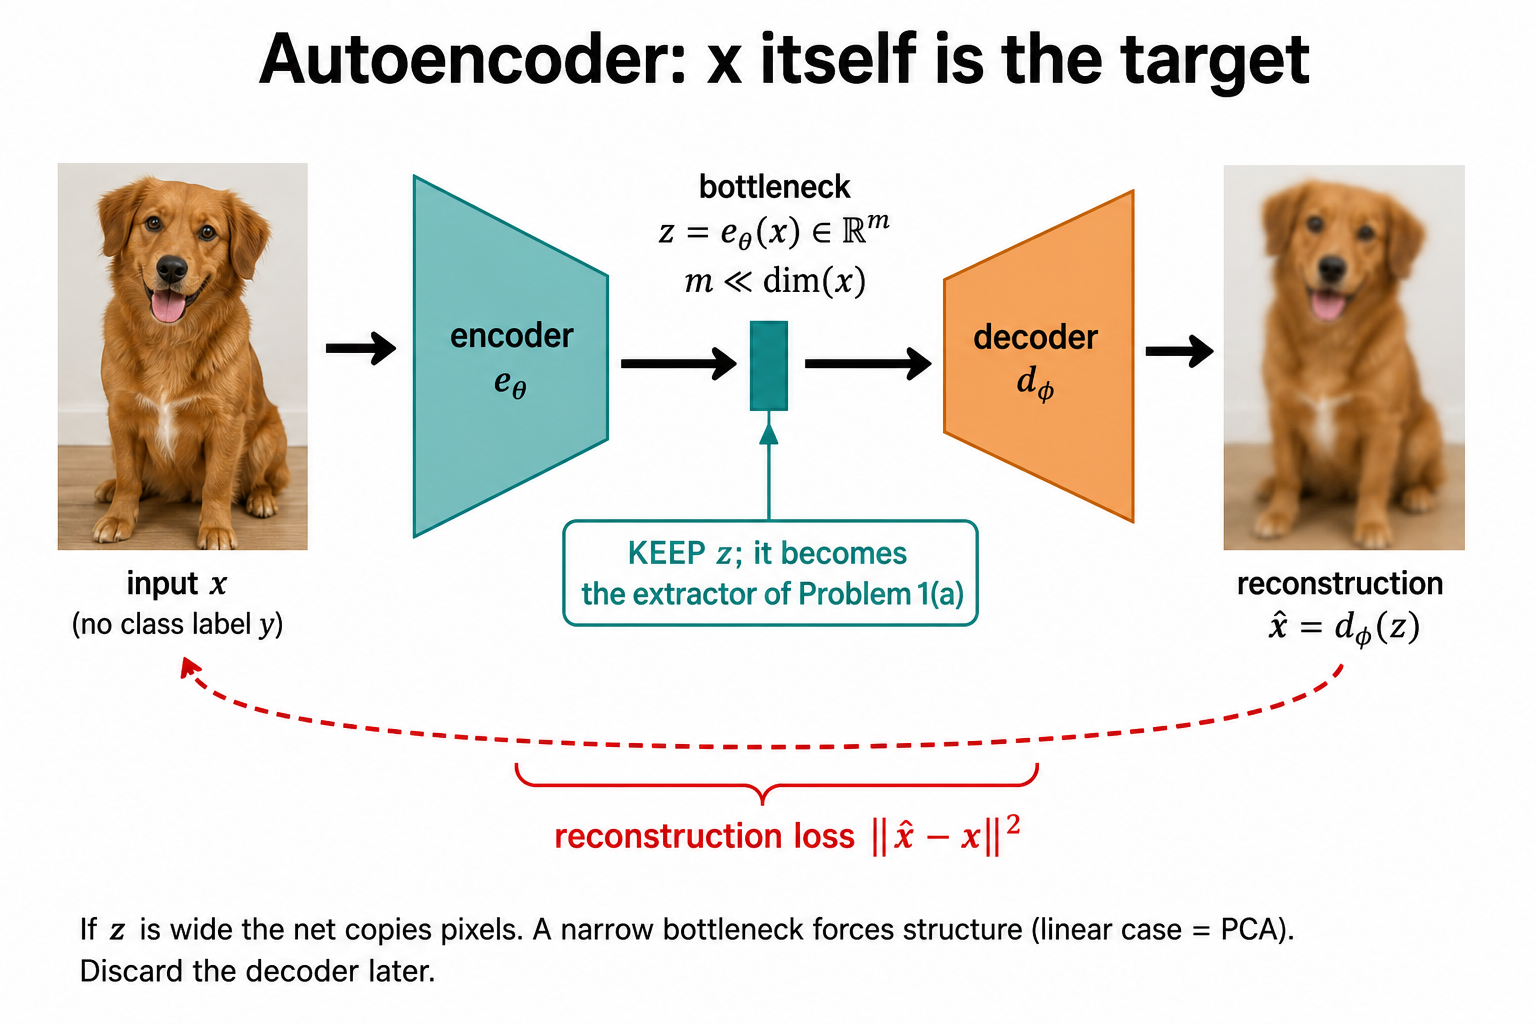
\includegraphics[width=0.96\linewidth]{figures/unsup/dlu-autoencoder.png}\\[0.35em]
{\small
Read the figure left to right as a closed loop that never uses a class \(y\).
The photograph \(x\) enters a teal encoder \(e_\theta\) and is compressed to a thin bottleneck \(z=e_\theta(x)\in\mathbb{R}^m\) with \(m\ll\dim x\).
An orange decoder \(d_\phi\) inverts that map and emits a reconstruction \(\widehat x=d_\phi(z)\).
The only training scalar is the red comparison under the pipeline: \(\|\widehat x-x\|^2\).
So \(x\) is its own target.
If \(z\) were as wide as \(x\), the pair could copy pixels and extract nothing; the narrow code forces a compressible structure (the linear case is PCA).
After training one discards \(d_\phi\) and keeps \(z\), which is then the feature extractor of Problem~1(a).
}
\end{center}

\begin{definition}[InfoNCE]
\label{def:dlu-infonce}
Given an anchor \(x\), a positive \(x^+\) (e.g.\ an augmented view), and negatives \(x_1^-,\dots,x_K^-\),
\[
\ell
=
-\log
\frac
{\exp\bigl(\langle z,z^+\rangle/\tau\bigr)}
{\exp\bigl(\langle z,z^+\rangle/\tau\bigr)+\sum_{k=1}^K\exp\bigl(\langle z,z_k^-\rangle/\tau\bigr)},
\]
where \(z,z^+,z_k^-\) are normalized embeddings and \(\tau>0\) is a temperature. This is a softmax classification of the positive among \(K+1\) candidates. The same identity appears in Part~D as a word-embedding / retrieval objective.
\end{definition}

\begin{center}
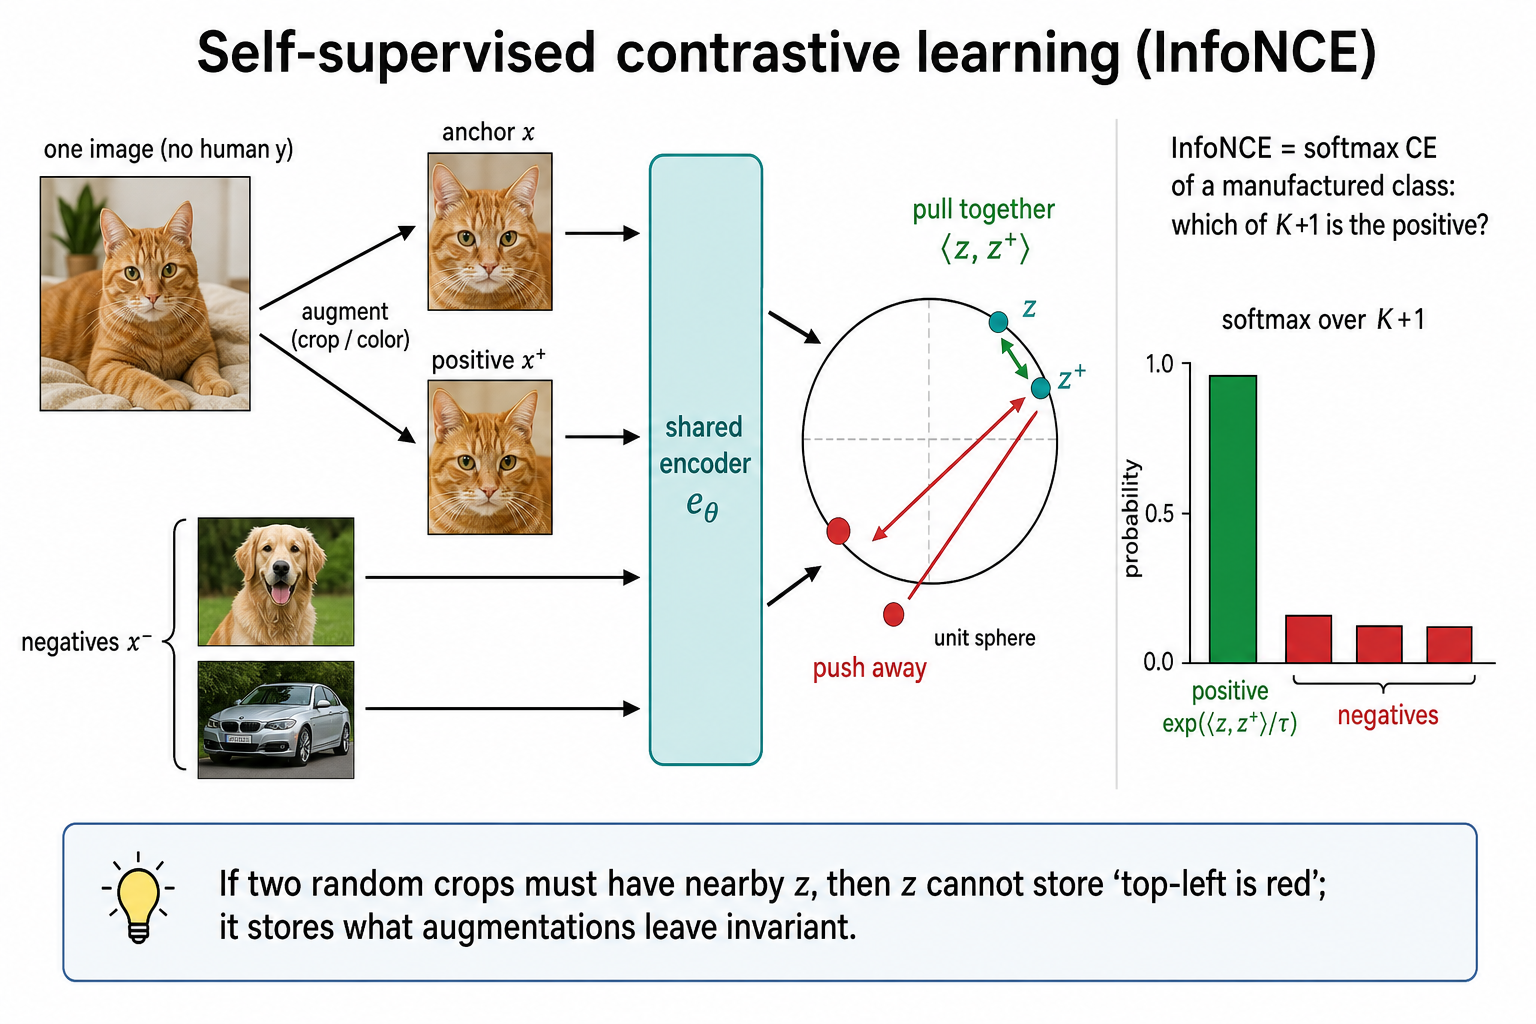
\includegraphics[width=0.96\linewidth]{figures/unsup/dlu-contrastive.png}\\[0.35em]
{\small
One unlabeled image (the cat) is turned into a manufactured classification problem.
Two random augmentations---a crop or a color jitter---produce an anchor \(x\) and a positive \(x^+\); other images in the batch are negatives \(x^-\).
A shared encoder \(e_\theta\) maps every view to a point on the unit sphere.
The green arrow pulls \(z\) toward \(z^+\); the red arrows push \(z\) away from each \(z^-\).
The right-hand bars are exactly InfoNCE: a softmax that asks ``which of the \(K+1\) candidates is the positive?'', with logits \(\langle z,z^+\rangle/\tau\) and \(\langle z,z_k^-\rangle/\tau\).
No human wrote ``cat''.
The invariance does the work: if two random crops must have nearby \(z\), then \(z\) cannot store ``the top-left pixel is red''; it can only store what the chosen augmentations leave unchanged.
}
\end{center}

\begin{remark}[Transfer is the extractor--head split]
\label{rem:dlu-transfer}
Pretrain \(e_{\theta_F}\) on reconstruction, contrastive pairs, or a large labeled source task; replace or retrain the classifier \(g_{\theta_G}\) on a target task with few labels. That is exactly the table in Problem~1 that distinguished the backbone from the head. Meta-learning (MAML-style) adds an inner loop that adapts \(\theta\) on a support set and an outer loop that scores the query set; later papers have not asked for the inner-loop algebra, only for the idea that the learning algorithm itself is the object being trained.
\end{remark}

\begin{center}
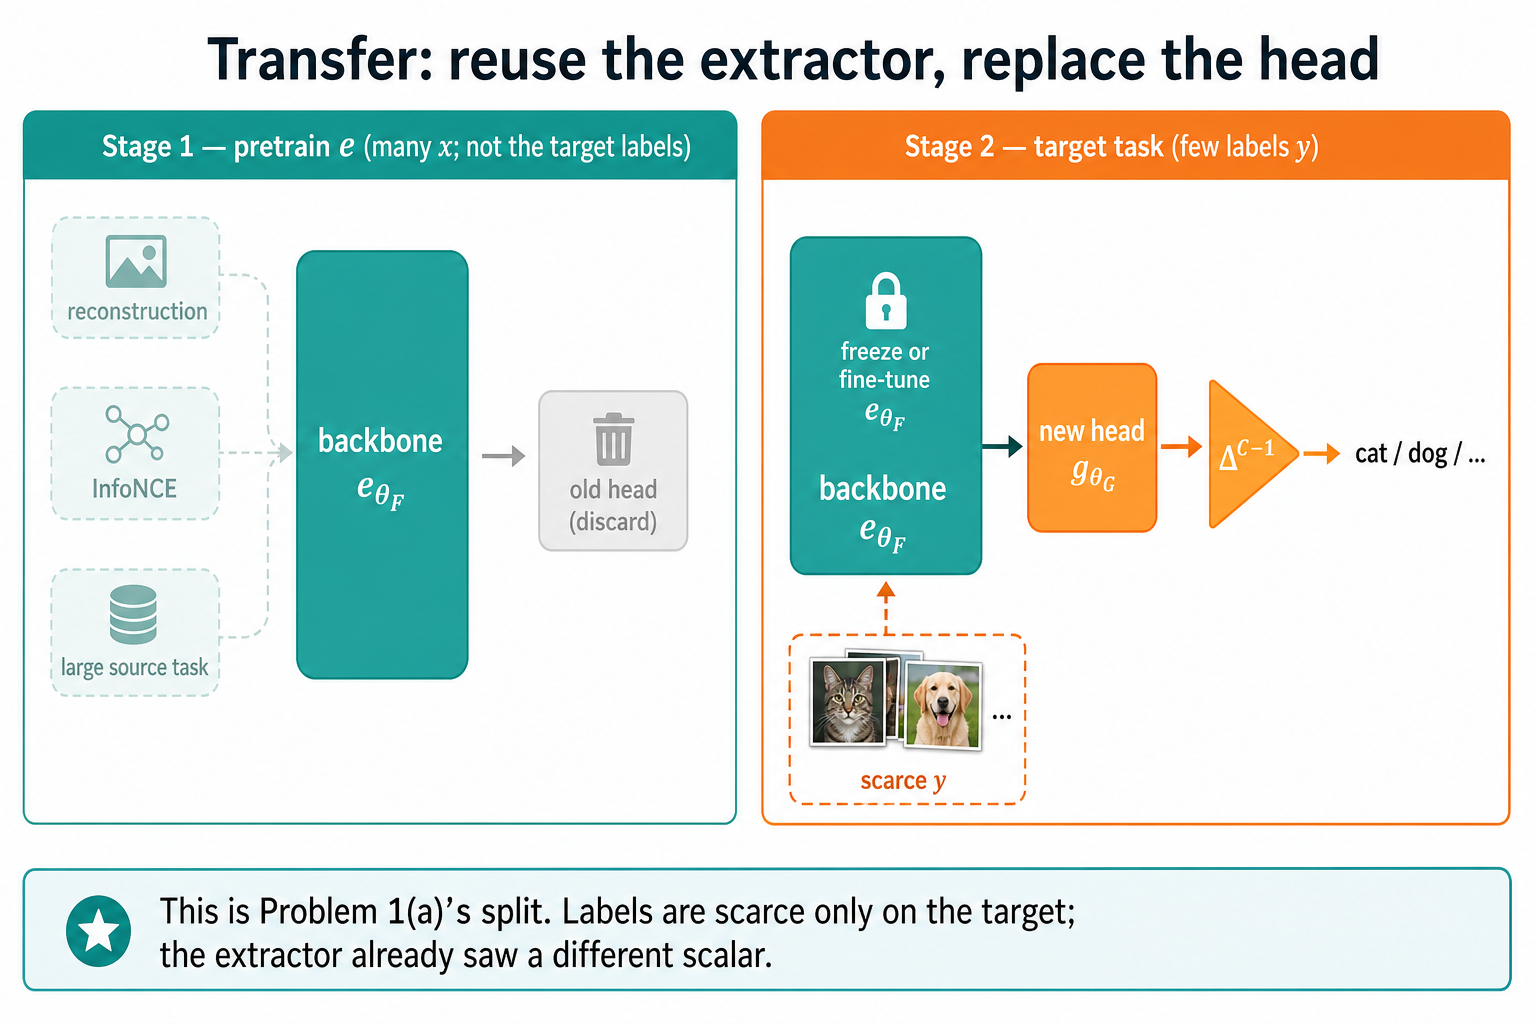
\includegraphics[width=0.96\linewidth]{figures/unsup/dlu-transfer.png}\\[0.35em]
{\small
The figure is two stages of the same split \(f=g_{\theta_G}\circ e_{\theta_F}\) already written in Problem~1(a).
Stage~1 trains the teal backbone \(e_{\theta_F}\) on many inputs \(x\), by reconstruction, by InfoNCE, or on a large source classification; the old head is discarded.
Stage~2 keeps that backbone (frozen or lightly fine-tuned) and attaches a new orange head \(g_{\theta_G}\) whose output is a simplex \(\Delta^{C-1}\) for the target classes.
The scarce labels \(y\) appear only on the right.
Transfer does not invent a fourth loss: it reuses an extractor that already saw a different scalar, and spends the few target labels on the head.
}
\end{center}

\begin{remark}[Implicit regularisation changes \(A(S)\), not the presence of \(y\)]
\label{rem:dlu-implicit-fig}
The last title word is the odd one. It is recorded here so the syllabus bullet is complete; it is not a way to train without labels. The figure below is the distinction already named in \cref{rem:dlu-two-reg}.
\end{remark}

\begin{center}
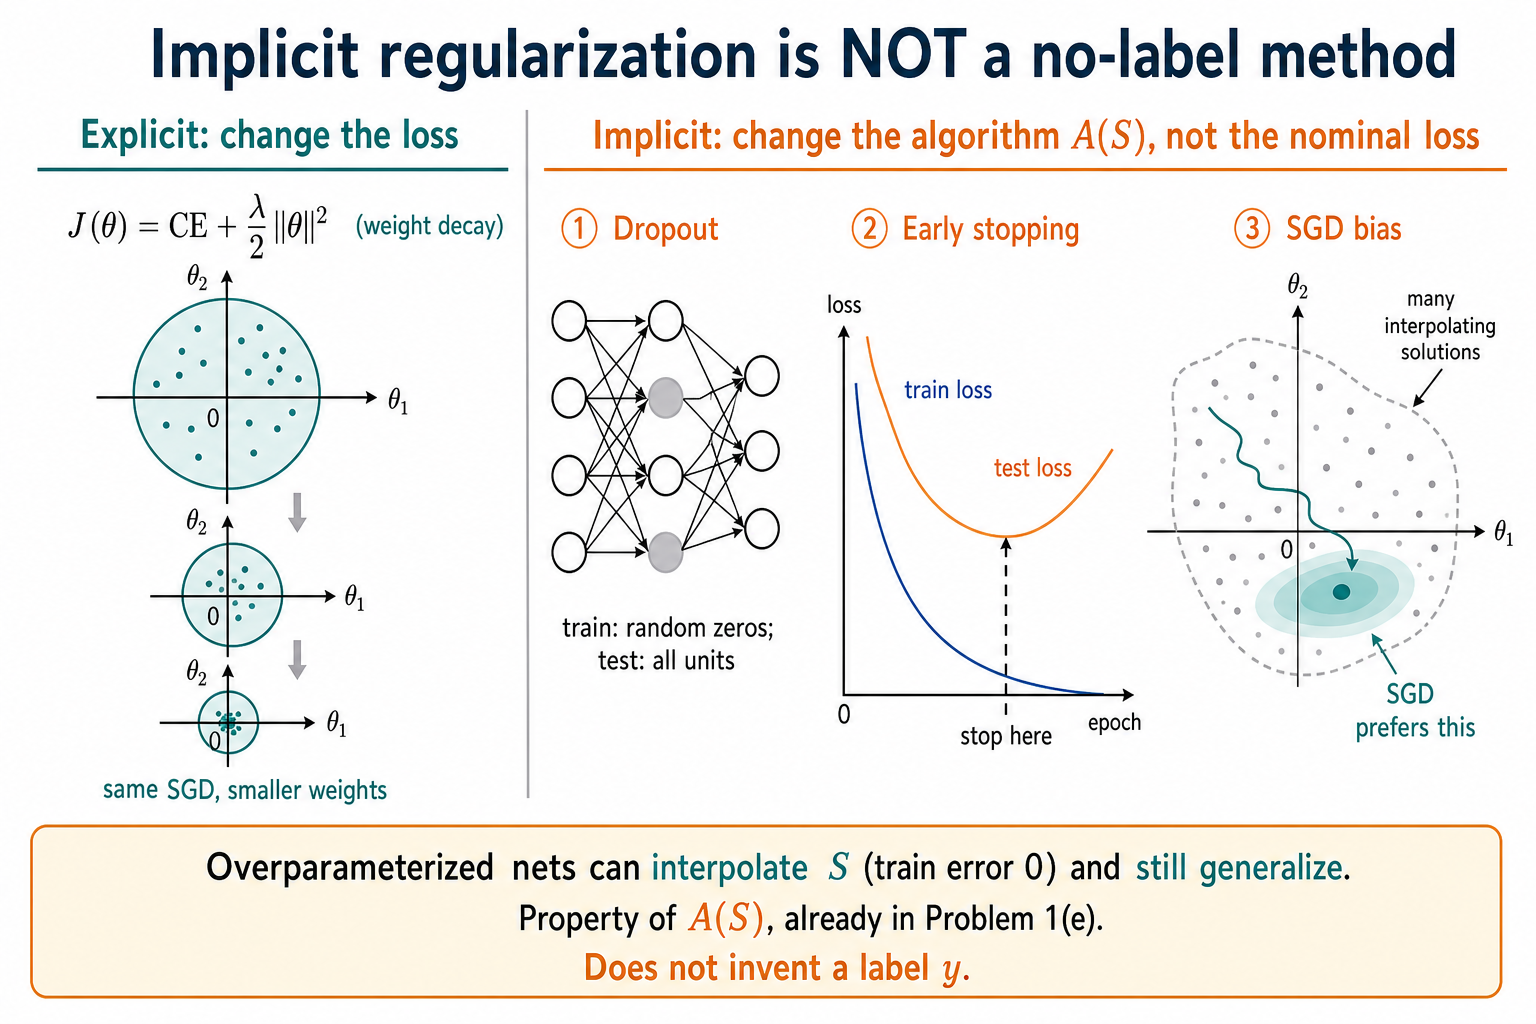
\includegraphics[width=0.96\linewidth]{figures/unsup/dlu-implicit-reg.png}\\[0.35em]
{\small
The left column is explicit regularisation: one adds \(\tfrac{\lambda}{2}\|\theta\|^2\) to the same classification loss, so SGD is asked for smaller weights.
The right column leaves the nominal loss unchanged and changes the algorithm \(A(S)\).
Dropout zeros random units at train time and uses all units at test time.
Early stopping cuts the run at the minimum of the test curve, before the train loss has finished interpolating.
SGD itself is biased among the many interpolating solutions of an overparameterized net; the path drawn in the figure prefers a flat basin.
The banner is the exam sentence: such a net can interpolate \(S\) (train error \(0\)) and still generalise.
That is a property of \(A(S)\), already the overfitting discussion of Problem~1(e).
It does not manufacture a label \(y\).
}
\end{center}

\begin{exercise}[Autoencoder versus Problem~1]
\label{ex:dlu-ae}
Take \(m=1\), \(\mathcal{X}=\mathbb{R}^2\), a linear encoder \(z=w^\top x\in\mathbb{R}\), and a linear decoder \(\widehat x=z u\) with \(\|u\|=1\). The reconstruction loss is \(\|uu^\top x-x\|^2\) after absorbing \(w\) into the same direction as \(u\). What one-dimensional subspace minimizes the loss, and why is this not the classifier of Problem~1?
\end{exercise}

\begin{solution}[Autoencoder versus Problem~1]
\(\|uu^\top x-x\|^2=\|x\|^2-\langle u,x\rangle^2\) for \(\|u\|=1\). Minimizing reconstruction is maximizing \(\langle u,x\rangle^2\), i.e.\ taking \(u\) along the top principal direction of this single point (or of the empirical covariance, if one averages over \(S\)). The output is a reconstruction in \(\mathcal{X}\), not a vector in \(\Delta^{C-1}\). Problem~1 needs labels; an autoencoder does not. After pretraining, one may freeze \(u\) (or \(e_\theta\)) and attach a new head, which is the transfer move of \cref{rem:dlu-transfer}.
\end{solution}


\subsubsection{Generative families: likelihood, flows, VAEs, GANs, and flow matching}
\label{subsubsec:dlu-gen}

The previous subsection trained a reusable map \(z=e(x)\). The object was the encoder; drawing a new \(x\) was not the point. This subsection trains a model of the law of \(x\) itself. The object is a density \(p_\theta\), or a sampler whose pushforward is close to \(p_{\mathrm{data}}\). There is still no class label \(y\). The scalar is no longer ``reconstruct \(x\)'' or ``agree on two views''; it is some computational stand-in for ``make \(p_\theta\) close to \(p_{\mathrm{data}}\)''.

The official syllabus item is ``visual generative models: GAN, VAE, diffusion, flows, expressivity''. Problem~2 is the continuous-time score case. Later papers ask for the cousins. The dictionary below is organised by \emph{what one can evaluate}, not by architecture names.

\begin{remark}[Generation is not representation]
\label{rem:dlu-gen-not-rep}
The previous subsection kept \(e\) and discarded the pretext head. This subsection must produce a new \(x\). A VAE looks like an autoencoder, but its decoder is a conditional density \(p_\theta(x\mid z)\) and its encoder is regularised toward a prior, so that drawing \(z\sim p(z)\) at test time is legal. An autoencoder that only reconstructs training points has no such licence. A GAN has no encoder at all. A flow has an inverse map only because invertibility is how one evaluates the density. Same unlabeled \(\{x_i\}\); different question.
\end{remark}

\begin{center}
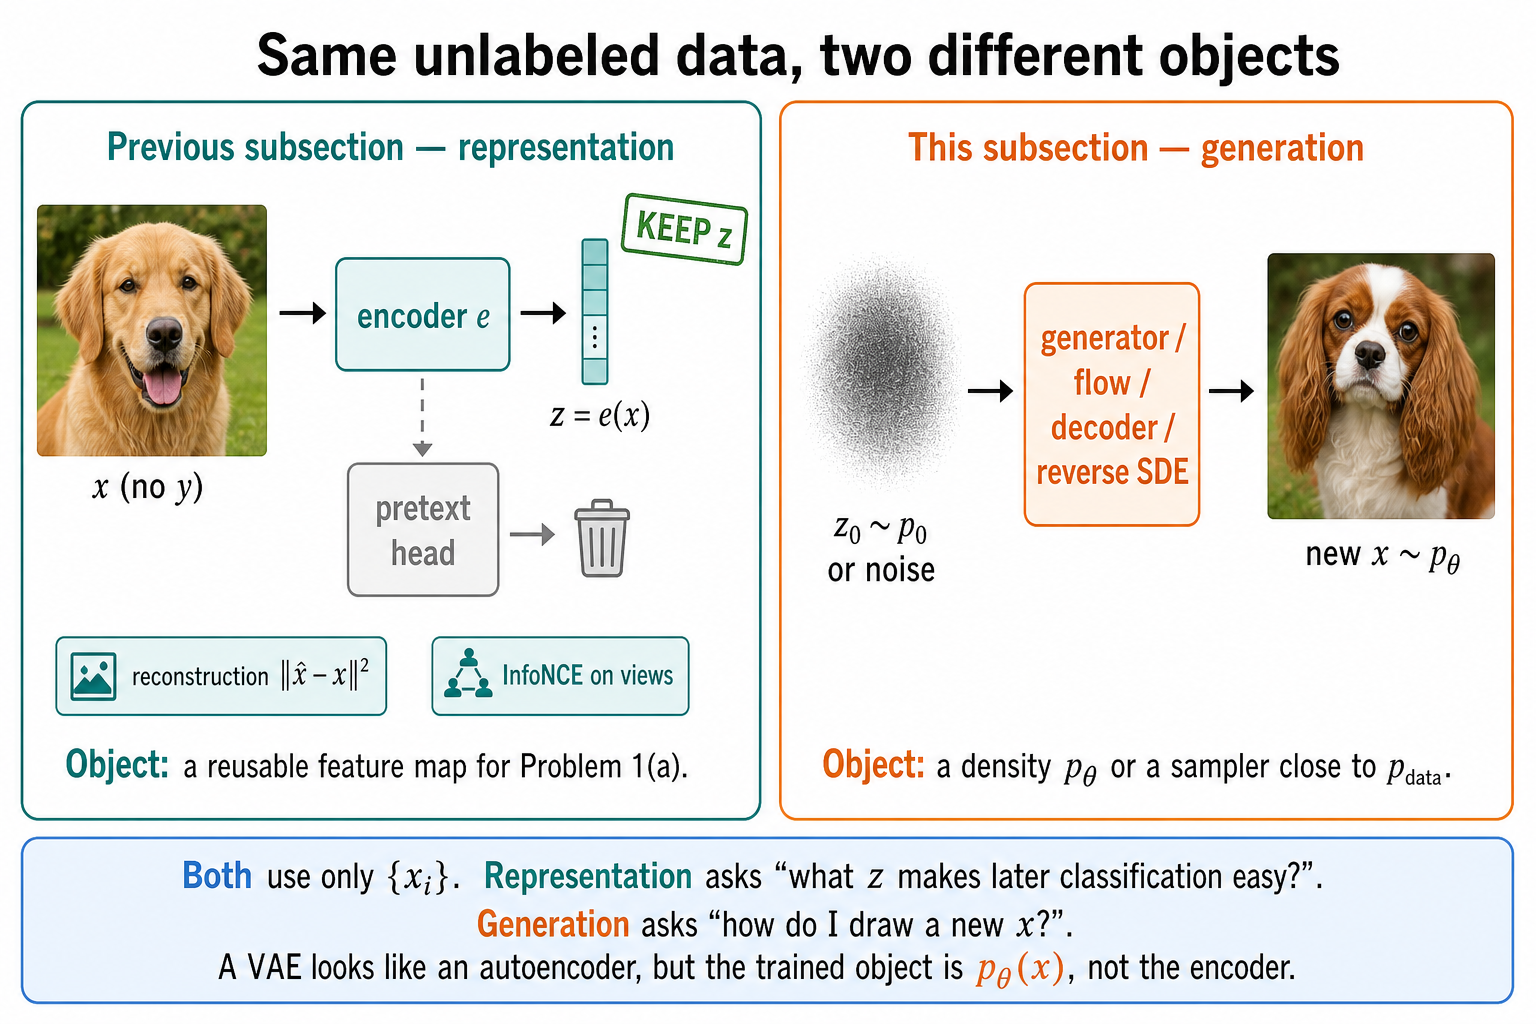
\includegraphics[width=0.96\linewidth]{figures/gen/dlu-gen-vs-rep.png}\\[0.35em]
{\small
Read the two columns as the same unlabeled photograph asked two different questions.
The teal column is the previous subsection: \(x\) is compressed to \(z=e(x)\), the pretext head is thrown away, and \(z\) is kept as the extractor of Problem~1(a).
The orange column is this subsection: one starts from noise or a base draw \(z_0\sim p_0\), pushes it through a generator / flow / decoder / reverse SDE, and obtains a \emph{new} \(x\sim p_\theta\).
The object on the right is a density or a sampler, not a feature map.
A VAE uses boxes that look like the autoencoder on the left; what it trains is the object on the right.
}
\end{center}

\begin{proposition}[Maximum likelihood is a KL]
\label{prop:dlu-mle-kl}
If \(p_{\mathrm{data}}\) and \(p_\theta\) are densities,
\[
\mathrm{KL}(p_{\mathrm{data}}\|p_\theta)
=
\mathbb{E}_{x\sim p_{\mathrm{data}}}\bigl[\log p_{\mathrm{data}}(x)-\log p_\theta(x)\bigr].
\]
The first summand does not depend on \(\theta\), so
\[
\arg\max_\theta\,\mathbb{E}_{x\sim p_{\mathrm{data}}}[\log p_\theta(x)]
=
\arg\min_\theta\,\mathrm{KL}(p_{\mathrm{data}}\|p_\theta).
\]
On a finite sample the left-hand side is ordinary ERM for the point loss \(\ell(\theta,x)=-\log p_\theta(x)\), the same \(L_S\) construction as in Part~A.
\end{proposition}

\begin{proof}
Expand the KL and drop \(\mathbb{E}[\log p_{\mathrm{data}}]\). The identity is an equality of objectives, not an approximation. It fails as a computational recipe whenever \(\log p_\theta(x)\) cannot be evaluated (the VAE and GAN cases below).
\end{proof}

\begin{remark}[The computational fork]
\label{rem:dlu-gen-fork}
If \(\log p_\theta(x)\) is cheap, train \(-\log p_\theta\) (a flow). If it is an intractable integral, maximise a lower bound (VAE, DDPM ELBO). If there is no density at all, play a game (GAN). If a marginal object is unknown but a conditional cousin is closed-form, regress onto the cousin (score matching, flow matching). The four stand-ins are not four different goals. The exam move is to name which scalar one can actually compute.
\end{remark}

\begin{center}
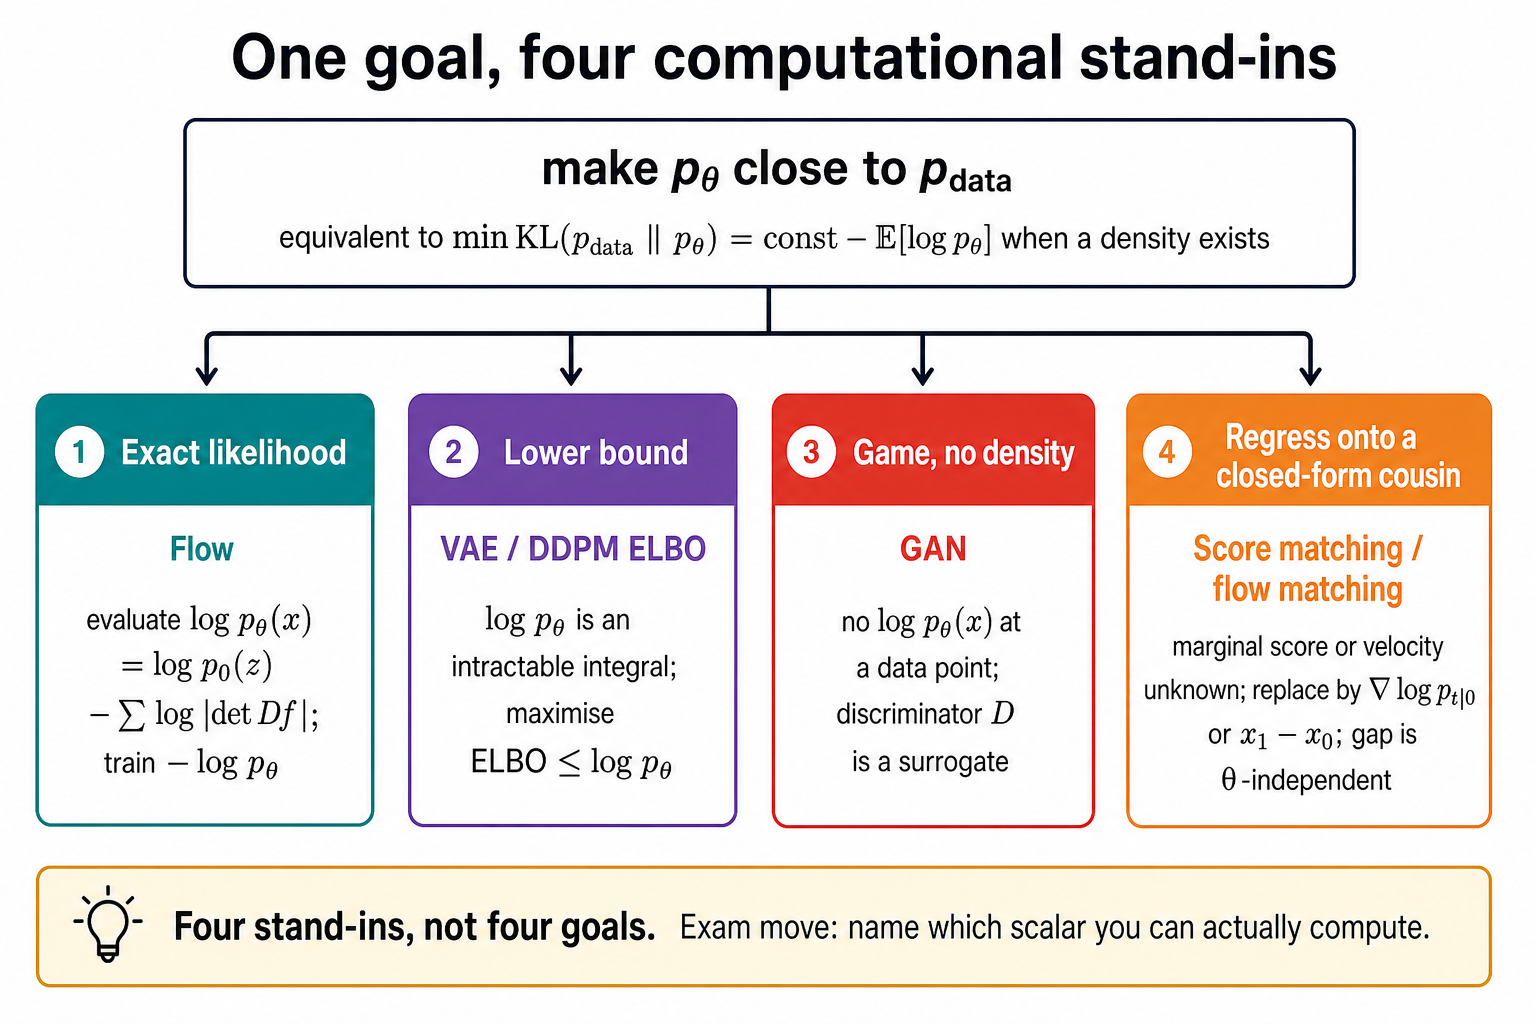
\includegraphics[width=0.96\linewidth]{figures/gen/dlu-gen-fork.png}\\[0.35em]
{\small
The top box is \cref{prop:dlu-mle-kl}: whenever a density exists, making \(p_\theta\) close to \(p_{\mathrm{data}}\) is the same as maximising \(\mathbb{E}[\log p_\theta]\).
The four cards are the four ways the rest of the subsection computes a stand-in for that expectation.
Teal: a flow evaluates \(\log p_\theta(x)\) exactly, paying a Jacobian at every invertible layer.
Purple: a VAE or a DDPM cannot evaluate the marginal, so it maximises an ELBO that sits below \(\log p_\theta\).
Red: a GAN never writes a density; the discriminator is a surrogate, not a rewrite of the KL.
Orange: Problem~2 and flow matching never need \(\log p_\theta\) either; they regress onto a closed-form conditional (a score or a velocity) whose gap to the desired marginal is \(\theta\)-independent.
}
\end{center}

\paragraph{Normalizing flows.}

\begin{proposition}[Change of variables]
\label{prop:dlu-flow}
Let \(z_0\sim p_0\) and \(z_\ell=f_\ell(z_{\ell-1})\) with each \(f_\ell\) a \(C^1\) diffeomorphism, and set \(x=z_L\). Then
\[
\log p_\theta(x)
=
\log p_0(z_0)
-
\sum_{\ell=1}^L\log\bigl\lvert\det Df_\ell(z_{\ell-1})\bigr\rvert,
\]
where \(z_0=f_1^{-1}\circ\cdots\circ f_L^{-1}(x)\) is obtained by running the inverses. The training loss on \(\{x^{(i)}\}_{i=1}^N\) is the Monte Carlo negative log-likelihood
\[
L_N(\theta)
=
-\frac1N\sum_{i=1}^N\log p_\theta\bigl(x^{(i)}\bigr).
\]
\end{proposition}

\begin{remark}[Why flows exist]
\label{rem:dlu-why-flow}
Problem~2 never evaluates \(p_t(x_t)\). A flow evaluates \(p_\theta(x)\) exactly, at the cost of designing invertible layers with cheap Jacobians. That is the opposite computational profile of score matching.
\end{remark}

\begin{center}
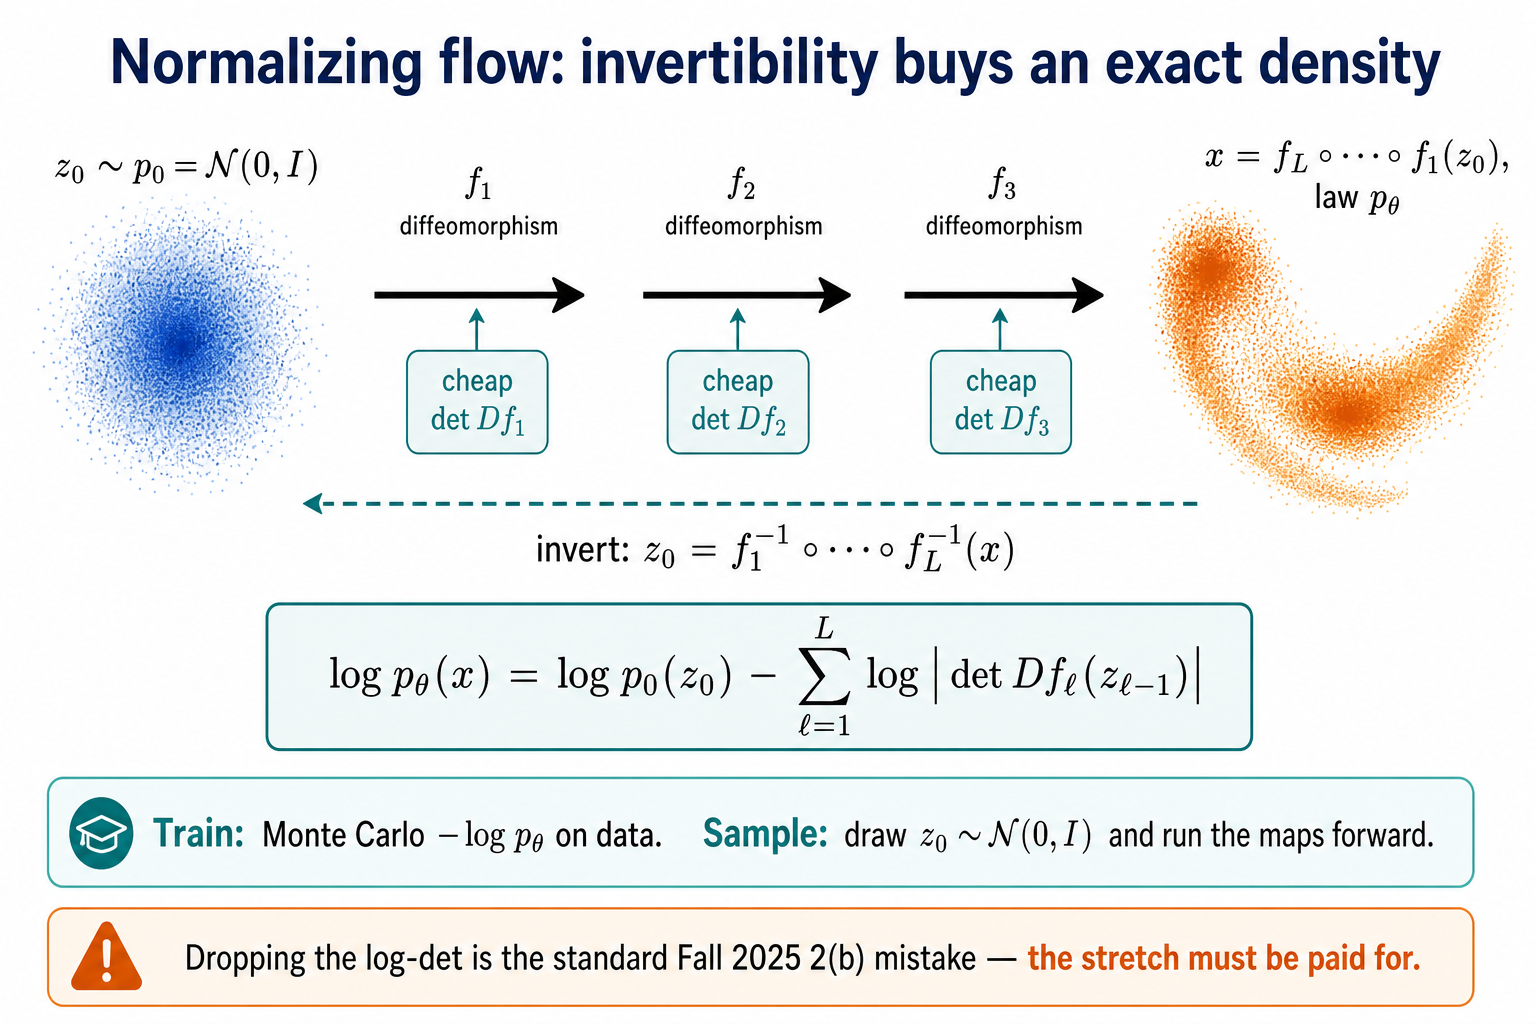
\includegraphics[width=0.96\linewidth]{figures/gen/dlu-gen-flow.png}\\[0.35em]
{\small
Start from a base Gaussian \(z_0\sim p_0\).
Each teal arrow is a \(C^1\) diffeomorphism \(f_\ell\) with a cheap Jacobian; the composition warps the round cloud into the data-shaped orange cloud, whose law is \(p_\theta\).
Because every layer is invertible, a data point \(x\) can be sent backward to a unique \(z_0\), and the change-of-variables formula of \cref{prop:dlu-flow} gives an exact number \(\log p_\theta(x)=\log p_0(z_0)-\sum_\ell\log\lvert\det Df_\ell\rvert\).
Training is ordinary Monte Carlo negative log-likelihood of that number.
Sampling is the forward maps: draw \(z_0\), apply \(f_1,\dots,f_L\).
The log-det term is the price of stretching the base measure; dropping it is the standard mistake on Fall 2025 Problem~2(b).
}
\end{center}

\paragraph{Variational autoencoders.}

\begin{definition}[ELBO]
\label{def:dlu-elbo}
A latent-variable model is \(p_\theta(x,z)=p_\theta(x\mid z)p(z)\). The marginal \(p_\theta(x)=\int p_\theta(x,z)\,dz\) is typically intractable. For any variational density \(q_\phi(z\mid x)\),
\[
\log p_\theta(x)
=
\mathrm{KL}\bigl(q_\phi(z\mid x)\,\|\,p_\theta(z\mid x)\bigr)
+
\underbrace{\mathbb{E}_{q_\phi(z\mid x)}\bigl[\log p_\theta(x\mid z)\bigr]
-
\mathrm{KL}\bigl(q_\phi(z\mid x)\,\|\,p(z)\bigr)}_{\mathrm{ELBO}(x;\theta,\phi)}.
\]
The KL on the first line is nonnegative, so the ELBO lower-bounds the log-likelihood. The first ELBO term is a reconstruction (decode \(z\sim q_\phi(\,\cdot\mid x)\) and score \(x\)); the second term keeps \(q_\phi(\,\cdot\mid x)\) near the prior and is the regularizer.
\end{definition}

\begin{note}[Derivation of the ELBO identity]
\label{note:dlu-elbo-der}
The displayed split is an identity, not a modelling assumption. By Bayes,
\[
p_\theta(z\mid x)
=
\frac{p_\theta(x,z)}{p_\theta(x)}
=
\frac{p_\theta(x\mid z)\,p(z)}{p_\theta(x)},
\]
so, pointwise in \(z\),
\[
\log p_\theta(x)
=
\log p_\theta(x,z)
-
\log p_\theta(z\mid x).
\]
The left side does not depend on \(z\). Take \(\mathbb{E}_{z\sim q_\phi(\,\cdot\mid x)}\) of both sides:
\[
\log p_\theta(x)
=
\mathbb{E}_q\bigl[\log p_\theta(x,z)\bigr]
-
\mathbb{E}_q\bigl[\log p_\theta(z\mid x)\bigr].
\]
Add and subtract \(\mathbb{E}_q[\log q_\phi(z\mid x)]\):
\[
\log p_\theta(x)
=
\mathbb{E}_q\bigl[\log p_\theta(x,z)-\log q_\phi(z\mid x)\bigr]
+
\mathbb{E}_q\bigl[\log q_\phi(z\mid x)-\log p_\theta(z\mid x)\bigr].
\]
The second expectation is \(\mathrm{KL}(q_\phi(z\mid x)\,\|\,p_\theta(z\mid x))\). The first is the ELBO. That is
\[
\log p_\theta(x)
=
\mathrm{KL}\bigl(q_\phi(\,\cdot\mid x)\,\|\,p_\theta(\,\cdot\mid x)\bigr)
+
\mathrm{ELBO}(x;\theta,\phi).
\]
The KL is nonnegative, with equality iff \(q_\phi(\,\cdot\mid x)=p_\theta(\,\cdot\mid x)\). Hence the ELBO lower-bounds the log-likelihood, and the gap is exactly how wrong the encoder is as an approximation to the true posterior.

Expand the joint \(p_\theta(x,z)=p_\theta(x\mid z)p(z)\) inside the first expectation:
\[
\mathrm{ELBO}
=
\mathbb{E}_q\bigl[\log p_\theta(x\mid z)\bigr]
-
\mathbb{E}_q\bigl[\log q_\phi(z\mid x)-\log p(z)\bigr]
=
\mathbb{E}_q\bigl[\log p_\theta(x\mid z)\bigr]
-
\mathrm{KL}\bigl(q_\phi(z\mid x)\,\|\,p(z)\bigr).
\]
That is the two-term form in \cref{def:dlu-elbo}: reconstruct \(x\) from \(z\sim q_\phi(\,\cdot\mid x)\), and keep \(q_\phi(\,\cdot\mid x)\) near the prior.
\end{note}

\begin{remark}[What \(q_\phi\) fits, and why one computes the ELBO]
\label{rem:dlu-elbo-logic}
The variational family is \(\{q_\phi(\,\cdot\mid x)\}_\phi\). Given \(x\), its target is the latent posterior \(p_\theta(z\mid x)\), not the joint \(p_\theta(x,z)\) and not a posterior over parameters \(p(\theta\mid x)\). The parameter \(\theta\) is not the random variable being inferred. Bayes writes
\[
p_\theta(z\mid x)
=
\frac{p_\theta(x\mid z)\,p(z)}{p_\theta(x)},
\]
so the numerator is available (decoder times prior) but the normalizer \(p_\theta(x)=\int p_\theta(x,z)\,dz\) is not. Hence \(p_\theta(z\mid x)\) has no closed form, and the posterior KL \(\mathrm{KL}(q_\phi(\,\cdot\mid x)\,\|\,p_\theta(\,\cdot\mid x))\) cannot be evaluated.

That posterior KL is the actual discrepancy between \(q_\phi\) and the inverted conditional. The ELBO is not that discrepancy. From \cref{note:dlu-elbo-der},
\[
\log p_\theta(x)
=
\mathrm{KL}\bigl(q_\phi(\,\cdot\mid x)\,\|\,p_\theta(\,\cdot\mid x)\bigr)
+
\mathrm{ELBO}(x;\theta,\phi).
\]
The two terms are complementary: for fixed \(\theta\), maximizing the ELBO in \(\phi\) is exactly minimizing the posterior KL. One computes the ELBO because it expands into objects that do not mention \(p_\theta(z\mid x)\):
\[
\mathrm{ELBO}
=
\mathbb{E}_{q_\phi(\,\cdot\mid x)}\bigl[\log p_\theta(x\mid z)\bigr]
-
\mathrm{KL}\bigl(q_\phi(z\mid x)\,\|\,p(z)\bigr).
\]
All expectations are under \(q_\phi(\,\cdot\mid x)\), not under the true posterior. Do not conflate the two KLs: \(\mathrm{KL}(q_\phi\,\|\,p_\theta(\,\cdot\mid x))\) is the intractable gap; \(\mathrm{KL}(q_\phi\,\|\,p(z))\) is the tractable regularizer inside the ELBO. The joint \(p_\theta(x,z)\) and \(q_\phi(z\mid x)\) live on different spaces, so there is no ``KL between \(q\) and the joint''.
\end{remark}

\begin{remark}[Why the VAE does not maximize likelihood directly]
\label{rem:dlu-why-vae}
The integral over \(z\) has no closed form for a deep decoder. One therefore maximizes a tractable lower bound. Equality holds iff \(q_\phi(z\mid x)=p_\theta(z\mid x)\). Problem~2's denoising score-matching identity is a cousin: there one replaces an intractable score \(\nabla\log p_t\) by a tractable conditional score, and the gap is a \(\theta\)-independent constant. Here the gap is a KL that still depends on \(\phi\).
\end{remark}

\begin{center}
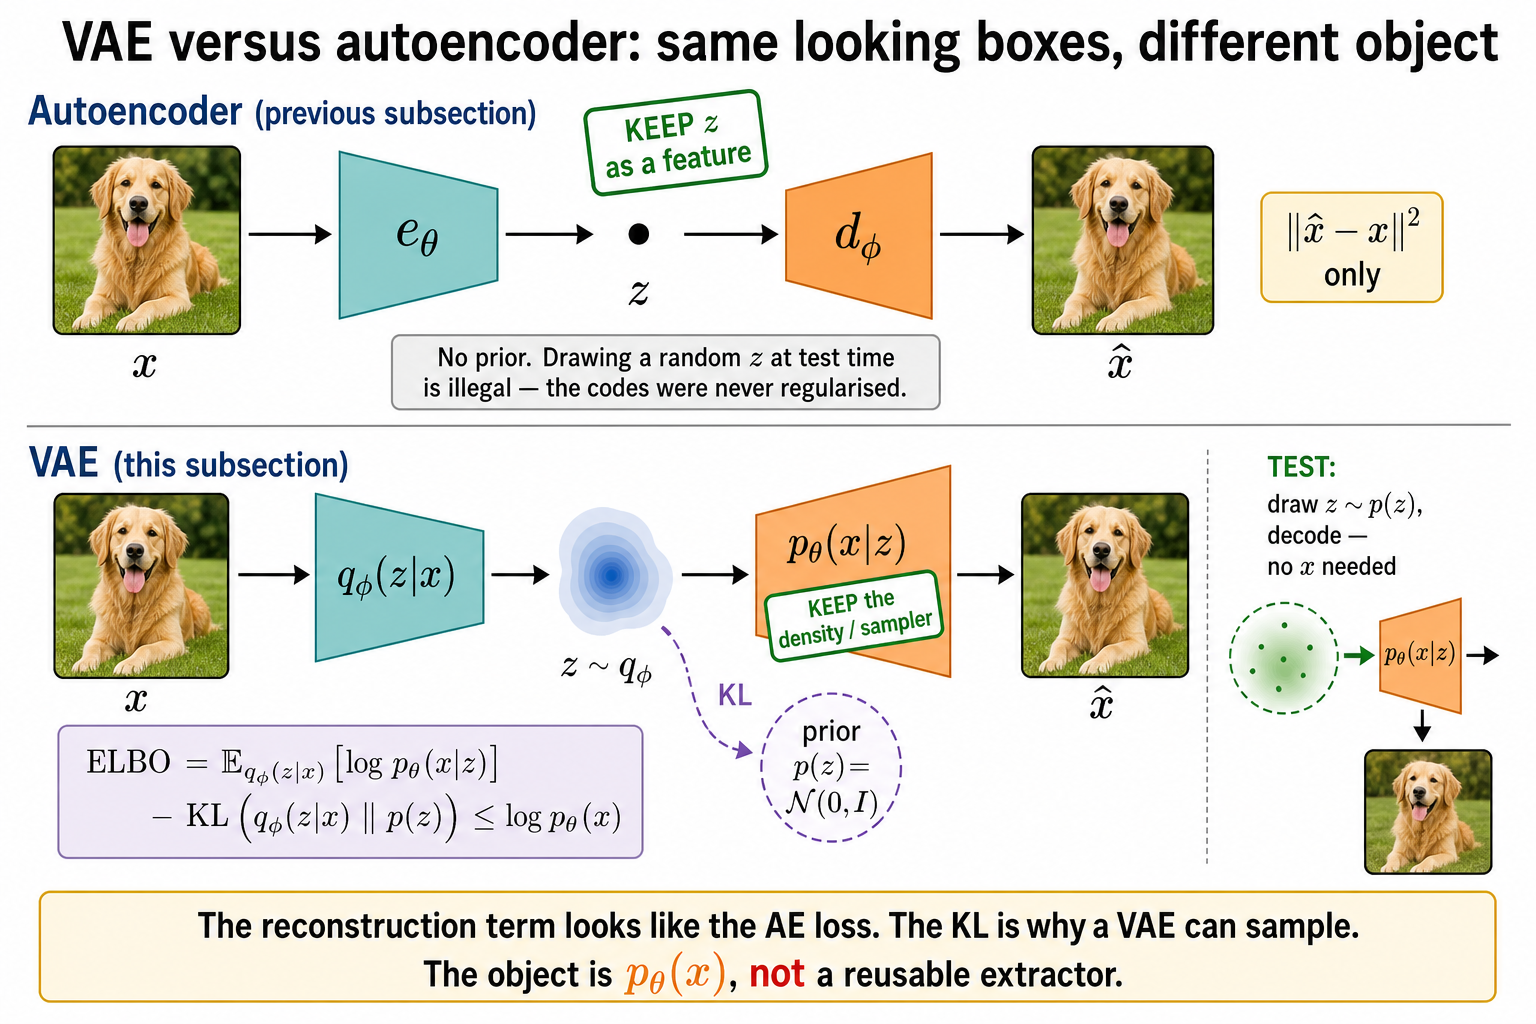
\includegraphics[width=0.96\linewidth]{figures/gen/dlu-gen-vae-vs-ae.png}\\[0.35em]
{\small
The two rows use the same three boxes. They are not the same object.
The top row is the autoencoder of the previous subsection: \(z\) is a point, the only scalar is \(\|\widehat x-x\|^2\), and one keeps the encoder as a feature.
There is no prior, so drawing a random code at test time is illegal---those codes were never regularised.
The bottom row is a VAE.
The encoder outputs a density \(q_\phi(z\mid x)\), not a point; the decoder is a conditional \(p_\theta(x\mid z)\); a prior \(p(z)\) sits beside them.
The ELBO of \cref{def:dlu-elbo} is reconstruction minus \(\mathrm{KL}(q_\phi(\,\cdot\mid x)\,\|\,p(z))\).
The KL is why one may sample: at test time draw \(z\sim p(z)\) and decode, with no \(x\) in hand.
The reconstruction term looks like the autoencoder loss; the object being trained is \(p_\theta(x)\), not a reusable extractor.
}
\end{center}

\paragraph{Discrete diffusion as a hierarchical VAE.}

\begin{proposition}[DDPM ELBO, exam form]
\label{prop:dlu-ddpm-elbo}
Let \(q(x_{1:T}\mid x_0)=\prod_{t=1}^T q(x_t\mid x_{t-1})\) with \(q(x_t\mid x_{t-1})=\mathcal{N}(\sqrt{\alpha_t}\,x_{t-1},\beta_t I)\) and \(\bar\alpha_t=\prod_{s=1}^t\alpha_s\). Let the reverse model be
\[
p_\theta(x_{0:T})
=
p(x_T)\prod_{t=1}^T p_\theta(x_{t-1}\mid x_t),
\]
with \(p(x_T)=\mathcal{N}(0,I)\) (or a close Gaussian). Then
\begin{align*}
\log p_\theta(x_0)
&\ge
-\mathrm{KL}\bigl(q(x_T\mid x_0)\,\|\,p(x_T)\bigr)
-\sum_{t=2}^T
\mathbb{E}_q\bigl[\mathrm{KL}\bigl(q(x_{t-1}\mid x_t,x_0)\,\|\,p_\theta(x_{t-1}\mid x_t)\bigr)\bigr]\\
&\qquad
+\mathbb{E}_q\bigl[\log p_\theta(x_0\mid x_1)\bigr].
\end{align*}
\end{proposition}

\begin{proofsketch}
This is the ELBO for the hierarchical latent variable \(x_{1:T}\) with encoder \(q(x_{1:T}\mid x_0)\) and decoder \(p_\theta(x_{0:T})\). Expanding
\[
\mathbb{E}_q\bigl[\log p_\theta(x_{0:T})-\log q(x_{1:T}\mid x_0)\bigr]
\]
and using the Markov structure of both chains produces a telescoping sum of KLs. The posterior \(q(x_{t-1}\mid x_t,x_0)\) is Gaussian and closed-form because the forward process is linear Gaussian; that is the discrete analogue of Problem~2's explicit \(p_{t\mid 0}\).
\end{proofsketch}

\begin{exercise}[Name the three ELBO pieces]
\label{ex:dlu-ddpm}
Write the reverse model \(p_\theta(x_{0:T})\). Then, without expanding every KL, name the three kinds of term in \cref{prop:dlu-ddpm-elbo} and say which posterior is closed-form.
\end{exercise}

\begin{solution}[Name the three ELBO pieces]
The reverse (decoder) factorization is
\[
p_\theta(x_{0:T})
=
p(x_T)\prod_{t=1}^T p_\theta(x_{t-1}\mid x_t),
\qquad
p(x_T)=\mathcal{N}(0,I).
\]
The ELBO of \cref{prop:dlu-ddpm-elbo} has three kinds of term: a terminal prior KL \(\mathrm{KL}(q(x_T\mid x_0)\,\|\,p(x_T))\); a sum of reverse-transition KLs \(\mathrm{KL}(q(x_{t-1}\mid x_t,x_0)\,\|\,p_\theta(x_{t-1}\mid x_t))\) for \(t=2,\dots,T\); and a reconstruction \(\mathbb{E}_q[\log p_\theta(x_0\mid x_1)]\). The encoder posterior \(q(x_{t-1}\mid x_t,x_0)\) is Gaussian and closed-form, because the forward process is linear Gaussian---the discrete analogue of Problem~2's \(p_{t\mid 0}\). That is Fall 2025 Problem~2(d).
\end{solution}

\begin{remark}[Two diffusion languages]
\label{rem:dlu-two-diffusions}
Problem~2 trains a score \(s_\theta(x_t,t)\approx\nabla\log p_t(x_t)\) by denoising score matching, using \(p_{t\mid 0}\). The display above trains reverse conditionals \(p_\theta(x_{t-1}\mid x_t)\) by a variational bound, using \(q(x_{t-1}\mid x_t,x_0)\). Under a VP discretization the two objectives become reparameterizations of each other (noise prediction versus score prediction), which is why Problem~2 already remarked that those targets are not unrelated. Fall 2025 Problem~2(d) wants the ELBO algebra, not the SDE.
\end{remark}

\paragraph{GANs.}

A flow evaluates \(\log p_\theta\); a VAE lower-bounds it. Both still sit on the likelihood side of \cref{prop:dlu-mle-kl}. An unrestricted generator \(G_\theta:z\mapsto x\) induces only a pushforward of \(p(z)\). That pushforward has no closed-form density in high dimension, so there is no \(\log p_\theta(x)\) to average and no latent posterior from which to write an ELBO. The Goodfellow game replaces the missing scalar by a second network that answers a binary question: ``is this \(x\) real?''. Training is alternating classification and fooling, not maximum likelihood.

\begin{definition}[GAN game]
\label{def:dlu-gan}
A generator \(G_\theta\) maps \(z\sim p(z)\) to \(x=G_\theta(z)\). Write \(p_G\) for the pushforward of \(p(z)\) through \(G_\theta\). A discriminator \(D_\psi:\mathcal{X}\to(0,1)\) is trained to distinguish draws from \(p_{\mathrm{data}}\) from draws from \(p_G\). The original game is
\[
\min_\theta\max_\psi\
V(G_\theta,D_\psi)
:=
\mathbb{E}_{x\sim p_{\mathrm{data}}}[\log D_\psi(x)]
+
\mathbb{E}_{z\sim p(z)}\bigl[\log\bigl(1-D_\psi(G_\theta(z))\bigr)\bigr].
\]
At an optimal discriminator the inner value is, up to the constant \(-\log 4\), twice the Jensen--Shannon divergence between \(p_{\mathrm{data}}\) and \(p_G\). There is no \(\log p_\theta(x)\) and no ELBO.
\end{definition}

\begin{note}[How to read the two expectations]
\label{note:dlu-gan-read}
Fix the generator and read \(V\) as binary cross-entropy for a classifier with labels \(\{0,1\}\). The first term is the log-likelihood that \(D_\psi\) assigns label \(1\) (``real'') to a true sample. The second is the log-likelihood that it assigns label \(0\) (``fake'') to \(G_\theta(z)\). The inner \(\max_\psi\) is ordinary logistic regression on a balanced mixture of reals and fakes. The outer \(\min_\theta\) freezes \(D_\psi\) and moves \(G_\theta\) so that those fakes are scored closer to \(1\). The two players do not share a likelihood; \(D_\psi\) is a surrogate critic, not a rewrite of \(\mathrm{KL}(p_{\mathrm{data}}\|p_G)\).
\end{note}

\begin{note}[Optimal discriminator and Jensen--Shannon]
\label{note:dlu-gan-js}
Rewrite the second expectation as an integral against \(p_G\). For a fixed generator the functional is
\[
V(D)
=
\int\Bigl(p_{\mathrm{data}}(x)\log D(x)+p_G(x)\log\bigl(1-D(x)\bigr)\Bigr)\,dx.
\]
The integrand, at each \(x\), is of the form \(a\log d+b\log(1-d)\) with \(a=p_{\mathrm{data}}(x)\), \(b=p_G(x)\), and \(d\in(0,1)\). The unique maximizer is \(d^*=a/(a+b)\), so
\[
D^*(x)
=
\frac{p_{\mathrm{data}}(x)}{p_{\mathrm{data}}(x)+p_G(x)}.
\]
Substitute \(D^*\) and rearrange to obtain
\[
V(D^*)
=
-\log 4
+
2\,\mathrm{JS}(p_{\mathrm{data}}\|p_G),
\]
where \(\mathrm{JS}(p\|q)=\frac12\mathrm{KL}(p\|m)+\frac12\mathrm{KL}(q\|m)\) and \(m=(p+q)/2\). That is the last sentence of \cref{def:dlu-gan}: after the inner max, the generator is asked to shrink a symmetric divergence between \(p_{\mathrm{data}}\) and \(p_G\). The identity is not a training recipe. One never computes \(D^*\) from the two densities (those densities are exactly what one does not have); one trains a network \(D_\psi\) to approximate the inner max, then takes a gradient step in \(\theta\).
\end{note}

\begin{remark}[What the game is for]
\label{rem:dlu-gan-use}
At test time the discriminator is discarded. Sampling is one forward map: draw \(z\sim p(z)\) and set \(x=G_\theta(z)\). There is no reverse SDE, no ancestral diffusion chain, and no encoder. That is why a GAN is cheap to sample and why \cref{prop:dlu-mle-kl} cannot be used as a loss: \(p_G(x)\) is not a number one can evaluate at a data point. The exam use of the display is comparative. Fall 2025 Problem~2 asked which scalar a flow or a VAE can compute; the matching sentence for a GAN is ``neither \(\log p_\theta\) nor an ELBO, only \(V(G,D)\)''. The same missing density is why a dropped mode does not appear in the loss---see \cref{rem:dlu-gan-collapse}.
\end{remark}

\begin{remark}[Mode collapse]
\label{rem:dlu-gan-collapse}
Because the generator is scored only through \(D_\psi\), it may concentrate on a few modes that already fool \(D_\psi\). Flows and VAEs cannot do that silently: a missing mode costs likelihood or reconstruction. Problem~2's score-matching objective is closer to the likelihood side of this dichotomy.
\end{remark}

\begin{center}
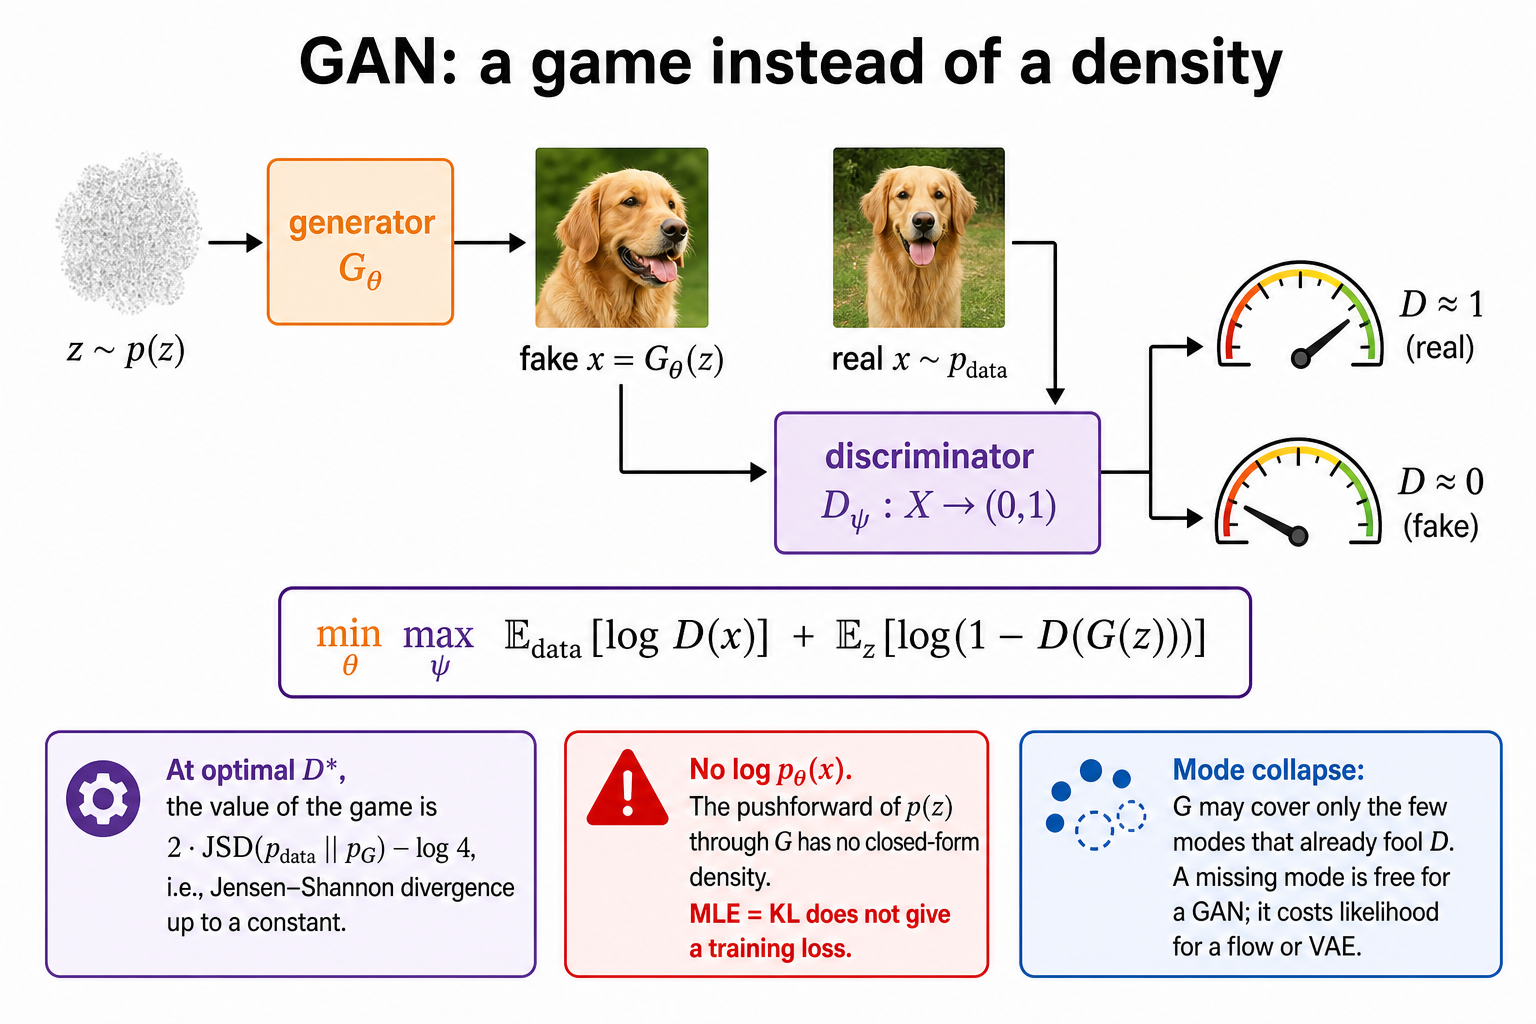
\includegraphics[width=0.96\linewidth]{figures/gen/dlu-gen-gan.png}\\[0.35em]
{\small
A latent \(z\sim p(z)\) is pushed through a generator \(G_\theta\) to a fake \(x\).
A discriminator \(D_\psi\) sees both that fake and a real draw from \(p_{\mathrm{data}}\), and is trained to output a number in \((0,1)\).
The original game of \cref{def:dlu-gan} is \(\min_\theta\max_\psi\); at an optimal \(D_\psi\) the inner value is a Jensen--Shannon divergence, up to a constant.
There is no \(\log p_\theta(x)\) and no ELBO: the pushforward of \(p(z)\) through a high-dimensional \(G_\theta\) has no closed-form density, so \cref{prop:dlu-mle-kl} does not give a training loss.
Mode collapse is the price of that freedom: \(G_\theta\) may cover only the modes that already fool \(D_\psi\).
A missing mode is free for a GAN and costly for a flow or a VAE.
}
\end{center}

\paragraph{Flow matching, the deterministic sibling of Problem~2.}

\begin{notation}[Interpolant]
\label{not:dlu-interp}
Let \(\pi_0\) be a base density (e.g.\ \(\mathcal{N}(0,I)\)) and \(\pi_1=p_{\mathrm{data}}\). Draw \((x_0,x_1)\sim\gamma\) with those marginals and set
\[
x_t=(1-t)x_0+t x_1,
\qquad
t\in[0,1].
\]
The conditional velocity is
\[
v_t(x_t\mid x_0,x_1)
:=
\frac{d}{dt}x_t
=
x_1-x_0.
\]
The marginal (population) velocity is the conditional expectation
\[
v_t(x)
:=
\mathbb{E}\bigl[v_t(x_t\mid x_0,x_1)\mid x_t=x\bigr].
\]
\end{notation}

\paragraph{Known, unknown, and the object one keeps.}

The data density \(\pi_1\) is never written in closed form; one has samples. The ODE is not a physical law. Its shape is already fixed by the interpolant of \cref{not:dlu-interp}. The ledger is then:

\begin{center}
{\footnotesize
\begin{tabularx}{\linewidth}{|p{4.4cm}|X|}
\hline
\textbf{Known (chosen or observed)} & \textbf{Where it comes from} \\ \hline
Base \(\pi_0\) & chosen, typically \(\mathcal{N}(0,I)\) \\ \hline
Data samples \(\{x_1^{(i)}\}\) & observed, from the unknown \(\pi_1\) \\ \hline
Coupling \(\gamma\) & chosen (independent pairing is enough) \\ \hline
Interpolant \(x_t=(1-t)x_0+tx_1\) & chosen (straight line) \\ \hline
Conditional velocity \(x_1-x_0\) & closed form, for each pair \\ \hline
Training triples \((t,x_t,x_1-x_0)\) & computed from the four rows above \\ \hline
\end{tabularx}
}
\end{center}

\begin{center}
{\footnotesize
\begin{tabularx}{\linewidth}{|p{4.4cm}|X|}
\hline
\textbf{Unknown (no closed form)} & \textbf{Why it is unavailable} \\ \hline
Data density \(\pi_1=p_{\mathrm{data}}\) & samples only \\ \hline
Intermediate law \(\pi_t=\mathrm{Law}(x_t)\) & many segments meet at the same \(x\) \\ \hline
Marginal velocity \(v_t(x)=\mathbb{E}[x_1-x_0\mid x_t=x]\) & a conditional expectation over those segments \\ \hline
Score \(\nabla\log\pi_t\) (Spring 2026(d)) & same unknown marginal \\ \hline
\end{tabularx}
}
\end{center}

One cannot regress onto \(v_t(x)\) itself: that is the unknown marginal object, exactly as \(\nabla\log p_t\) is unknown in Problem~2. The object one \emph{keeps} is a network \(v_\theta(t,x)\) whose population minimizer equals \(v_t\). The device is regression onto the known pair velocity:
\[
\mathbb{E}\bigl\|v_\theta(t,x_t)-(x_1-x_0)\bigr\|^2.
\]
At test time draw \(x_0\sim\pi_0\) and integrate \(\dot x=v_\theta\) to \(t=1\). There is no classifier and no explicit table of \(p_{\mathrm{data}}(x)\). The pipeline is
\[
\underbrace{\pi_0,\;x_1,\;x_t,\;x_1-x_0}_{\text{known}}
\;\longrightarrow\;
\underbrace{v_\theta\approx v_t}_{\text{learned}}
\;\longrightarrow\;
\underbrace{x_1^{\mathrm{new}}=\mathrm{ODE}(x_0;v_\theta)}_{\text{used to sample}}.
\]

\begin{proposition}[Continuity equation]
\label{prop:dlu-continuity}
If particles follow \(\frac{d}{dt}x_t=v_t(x_t)\) with \(v_t\) as in \cref{not:dlu-interp}, the law \(\pi_t\) of \(x_t\) satisfies
\[
\partial_t\pi_t+\nabla\cdot(\pi_t v_t)=0.
\]
In particular \(\pi_0\) is transported to \(\pi_1\).
\end{proposition}

\begin{proof}
The linear interpolant \(x_t=(1-t)x_0+tx_1\) has law \(\pi_t\) by construction, with \(\pi_1\) equal to the data marginal of \(\gamma\). The continuity (Liouville) equation is the infinitesimal conservation of mass for any ODE \(\dot x=v_t(x)\): for a test function \(\varphi\),
\[
\frac{d}{dt}\mathbb{E}[\varphi(x_t)]
=
\mathbb{E}\bigl[\langle\nabla\varphi(x_t),v_t(x_t)\rangle\bigr],
\]
which is the weak form of \(\partial_t\pi_t+\nabla\cdot(\pi_t v_t)=0\). The same identity holds with the \emph{conditional} velocity inside the expectation; taking \(\mathbb{E}[\,\cdot\mid x_t]\) replaces it by \(v_t(x_t)\) and does not change the marginal ODE.
\end{proof}

\begin{proposition}[Conditional flow-matching regression]
\label{prop:dlu-cfm}
The squared loss
\[
\mathcal{L}(\theta)
=
\mathbb{E}_{t,x_0,x_1}
\bigl\|
v_\theta(t,x_t)-(x_1-x_0)
\bigr\|^2
\]
is minimized (in \(L^2(\pi_t)\), for each \(t\)) at \(v_\theta(t,\,\cdot\,)=v_t\). Indeed, for each frozen \((t,x)\),
\[
\mathbb{E}\bigl[\|u-(x_1-x_0)\|^2\mid x_t=x\bigr]
=
\|u-v_t(x)\|^2
+
\mathrm{const}(t,x),
\]
so the unique minimizer in \(u\) is the conditional expectation \(v_t(x)\).
\end{proposition}

\begin{remark}[Same orthogonality as Problem~2]
\label{rem:dlu-same-ortho}
Problem~2(b) replaced \(\nabla\log p_t(x_t)\) by \(\nabla\log p_{t\mid 0}(x_t\mid x_0)\) and obtained a \(\theta\)-independent gap. Flow matching replaces \(v_t(x)\) by \(x_1-x_0\) and obtains the same kind of gap. In both cases one regresses onto a \emph{conditional} target that is known in closed form, and the population minimizer is the desired marginal object.
\end{remark}

\begin{center}
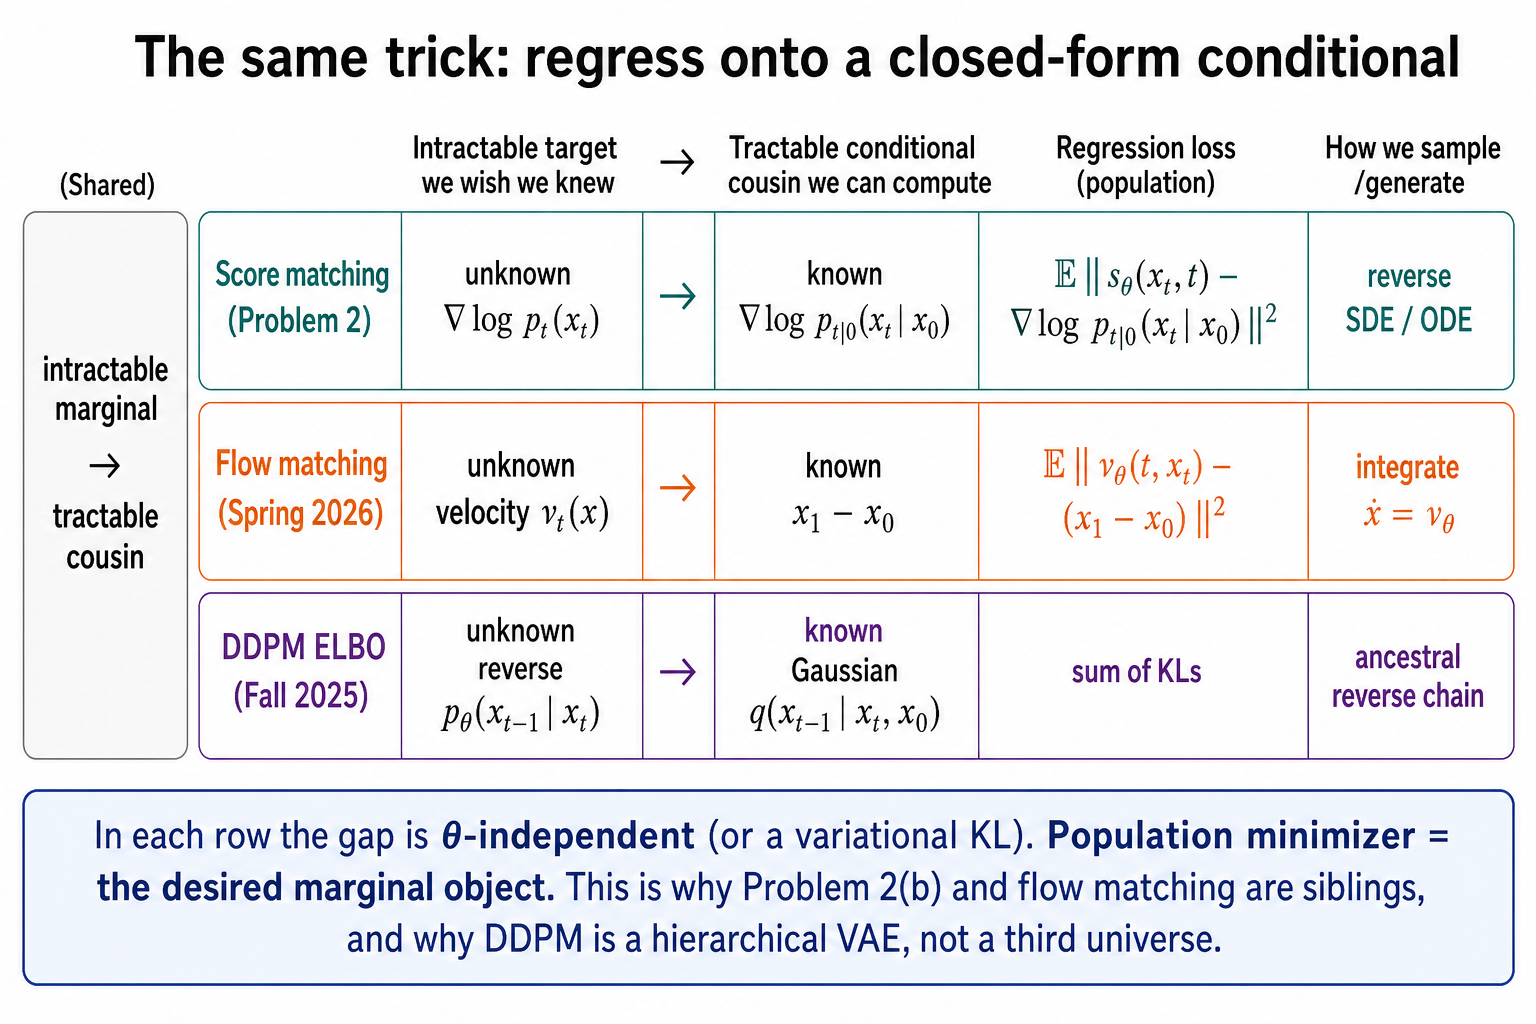
\includegraphics[width=0.96\linewidth]{figures/gen/dlu-gen-conditional.png}\\[0.35em]
{\small
The three rows are one trick written in three exam languages.
Row~1 is Problem~2: the marginal score \(\nabla\log p_t\) is unknown, the conditional score \(\nabla\log p_{t\mid 0}\) is Gaussian and closed-form, and denoising score matching regresses onto the latter.
Row~2 is Spring 2026 flow matching: the marginal velocity \(v_t(x)\) is unknown, the pair velocity \(x_1-x_0\) is elementary, and one regresses onto the pair.
Row~3 is Fall 2025 DDPM: the reverse conditional \(p_\theta(x_{t-1}\mid x_t)\) is unknown, the forward posterior \(q(x_{t-1}\mid x_t,x_0)\) is Gaussian, and the ELBO is a sum of KLs against that posterior.
In the first two rows the gap is \(\theta\)-independent; in the third it is a variational KL.
The population minimizer is the desired marginal object.
That is why Problem~2(b) and flow matching are siblings, and why a DDPM is a hierarchical VAE rather than a third universe.
}
\end{center}

\begin{proposition}[A score-corrected SDE with the same marginals]
\label{prop:dlu-sde-same}
The SDE
\[
dx_t
=
\bigl(v_t(x_t)+\beta_t\nabla\log\pi_t(x_t)\bigr)\,dt
+
\sqrt{2\beta_t}\,dW_t
\]
has Fokker--Planck equation
\[
\partial_t\pi
=
-\nabla\cdot\bigl(\pi(v_t+\beta_t\nabla\log\pi)\bigr)
+
\beta_t\Delta\pi,
\]
which reduces to \(\partial_t\pi+\nabla\cdot(\pi v_t)=0\) because \(\pi\nabla\log\pi=\nabla\pi\). Thus the SDE and the ODE share the family \(\{\pi_t\}\). In practice \(\nabla\log\pi_t\) is unknown and is replaced by a score network trained as in Problem~2.
\end{proposition}

\begin{center}
{\footnotesize
\begin{tabularx}{\linewidth}{|p{2.4cm}|X|X|X|}
\hline
\textbf{Family} & \textbf{What is tractable?} & \textbf{Training target} & \textbf{Sampling} \\ \hline
Flow & exact \(\log p_\theta(x)\) & \(-\log p_\theta\) (Jacobian) & invert the map \\ \hline
VAE & ELBO, not \(\log p_\theta\) & reconstruction \(-\) KL & decode \(z\sim p(z)\) \\ \hline
GAN & no likelihood & discriminator game & one forward \(G(z)\) \\ \hline
Score SDE (P2) & conditional score \(p_{t\mid 0}\) & denoising score matching & reverse SDE / ODE \\ \hline
DDPM ELBO & \(q(x_{t-1}\mid x_t,x_0)\) & reverse-conditionals via KL & ancestral reverse chain \\ \hline
Flow matching & conditional velocity \(x_1-x_0\) & \(L^2\) regression & integrate \(\dot x=v_\theta\) \\ \hline
\end{tabularx}
}
\end{center}

\begin{exercise}[MLE equals KL]
\label{ex:dlu-mle}
Prove \cref{prop:dlu-mle-kl} from the definition of KL, and explain why the same identity does \emph{not} give a training loss for a GAN generator.
\end{exercise}

\begin{solution}[MLE equals KL]
By definition
\[
\mathrm{KL}(p_{\mathrm{data}}\|p_\theta)
=
\int p_{\mathrm{data}}(x)\log\frac{p_{\mathrm{data}}(x)}{p_\theta(x)}\,dx
=
\mathbb{E}_{p_{\mathrm{data}}}[\log p_{\mathrm{data}}]
-
\mathbb{E}_{p_{\mathrm{data}}}[\log p_\theta].
\]
The first expectation is constant in \(\theta\). Minimizing the KL is therefore the same as maximizing \(\mathbb{E}[\log p_\theta]\). On a sample one replaces the expectation by an average, which is ERM for \(\ell(\theta,x)=-\log p_\theta(x)\).

A GAN generator does not furnish a density \(p_\theta(x)\) that one can evaluate at a data point (the pushforward of \(p(z)\) through a high-dimensional map has no closed-form density). There is therefore no \(\log p_\theta(x^{(i)})\) to average. The discriminator is a surrogate, not a rewrite of this KL.
\end{solution}

\begin{exercise}[A one-step flow]
\label{ex:dlu-flow-1}
Let \(d=1\), \(z\sim\mathcal{N}(0,1)\), and \(x=f(z)=2z+3\). Write \(\log p(x)\) from \cref{prop:dlu-flow} and check it against the known density of \(\mathcal{N}(3,4)\).
\end{exercise}

\begin{solution}[A one-step flow]
Here \(L=1\), \(f'(z)=2\), \(z=(x-3)/2\), and \(\log p_0(z)=-\frac12 z^2-\frac12\log(2\pi)\). The change-of-variables formula gives
\[
\log p(x)
=
-\frac12\Bigl(\frac{x-3}{2}\Bigr)^2
-\frac12\log(2\pi)
-\log 2
=
-\frac{(x-3)^2}{8}
-\frac12\log(2\pi\cdot 4),
\]
which is exactly \(\log\mathcal{N}(x;3,4)\). The \(-\log\lvert\det Df\rvert\) term is the whole difference between ``ignore the stretching'' and a correctly normalized density. Dropping it is the standard mistake on Fall 2025 Problem~2(b).
\end{solution}

\begin{exercise}[ELBO terms in words]
\label{ex:dlu-elbo-words}
For a VAE, identify which term of \cref{def:dlu-elbo} encourages \(d_\phi\circ e_\theta\) to reconstruct \(x\), and which term prevents the encoder from using a different latent code for every training point. Why is the ELBO not equal to \(\log p_\theta(x)\) in general?
\end{exercise}

\begin{solution}[ELBO terms in words]
The reconstruction term \(\mathbb{E}_{q_\phi(z\mid x)}[\log p_\theta(x\mid z)]\) is large when decoded samples from the encoder land near \(x\). The KL \(\mathrm{KL}(q_\phi(z\mid x)\,\|\,p(z))\) is large when the encoder posterior is far from the prior (typically \(\mathcal{N}(0,I)\)); minimizing it (as part of maximizing the ELBO) stops the encoder from encoding each \(x\) as a disjoint delta, which would make the latent space unusable at test time (when one samples \(z\sim p(z)\), not \(z\sim q_\phi(\,\cdot\mid x)\)).

The ELBO equals \(\log p_\theta(x)\) if and only if \(q_\phi(z\mid x)=p_\theta(z\mid x)\). A finitely parameterized encoder does not match the true posterior, so the gap \(\mathrm{KL}(q_\phi\|p_\theta(\,\cdot\mid x))\) is positive. That is why Fall 2025 Problem~2(c) asks for a lower bound and not an identity.
\end{solution}

\begin{exercise}[Conditional velocity and the regression target]
\label{ex:dlu-cfm-num}
Take \(d=1\), \(x_0=0\), \(x_1=4\), and \(t=1/4\). Compute \(x_t\) and \(v_t(x_t\mid x_0,x_1)\). Then, without computing any integral, explain why the population minimizer of \(\mathbb{E}[(u-(x_1-x_0))^2\mid x_t=1]\) is not necessarily \(4\) if other pairs \((x_0,x_1)\) can also produce \(x_t=1\).
\end{exercise}

\begin{solution}[Conditional velocity and the regression target]
The interpolant is \(x_t=(1-t)x_0+tx_1=(3/4)\cdot 0+(1/4)\cdot 4=1\). The conditional velocity is \(x_1-x_0=4\).

If this pair were the only pair yielding \(x_t=1\), the conditional expectation \(v_t(1)\) would be \(4\). In general many segments pass through the same point: e.g.\ \((x_0,x_1)=(-1,7)\) also gives \(x_{1/4}=1\), with velocity \(8\). The population target \(v_t(1)\) is the average of all such velocities, weighted by the posterior of \((x_0,x_1)\) given \(x_t=1\). That averaging is \cref{prop:dlu-cfm}. It is the same reason Problem~2's \(\nabla\log p_t(x_t)\) is an average of \(\nabla\log p_{t\mid 0}(x_t\mid x_0)\) and not a single-pair score.
\end{solution}

\begin{exercise}[The Fokker--Planck cancellation]
\label{ex:dlu-fp}
Starting from the Fokker--Planck operator for \(dx=\mu\,dt+\sqrt{2\beta}\,dW\), show that \(\mu=v+\beta\nabla\log\pi\) cancels the extra terms and leaves \(\partial_t\pi+\nabla\cdot(\pi v)=0\). (You may assume \(\pi>0\) and write \(\nabla\log\pi=\nabla\pi/\pi\).)
\end{exercise}

\begin{solution}[The Fokker--Planck cancellation]
For the SDE \(dx=\mu\,dt+\sqrt{2\beta}\,dW\), Fokker--Planck reads
\[
\partial_t\pi
=
-\nabla\cdot(\mu\pi)
+
\beta\Delta\pi.
\]
Substitute \(\mu=v+\beta\nabla\log\pi\):
\[
\nabla\cdot(\mu\pi)
=
\nabla\cdot(\pi v)
+
\beta\nabla\cdot(\pi\nabla\log\pi)
=
\nabla\cdot(\pi v)
+
\beta\nabla\cdot(\nabla\pi)
=
\nabla\cdot(\pi v)
+
\beta\Delta\pi.
\]
Hence
\[
\partial_t\pi
=
-\nabla\cdot(\pi v)-\beta\Delta\pi+\beta\Delta\pi
=
-\nabla\cdot(\pi v).
\]
The score drift is exactly the It\^o correction that cancels the Laplacian. This is why Spring 2026 Problem~2(d) can claim that the SDE and the ODE share \(\{\pi_t\}\), and why the unknown \(\nabla\log\pi_t\) may be replaced by the score network already trained in Problem~2.
\end{solution}

\begin{remark}[Engineering gaps left as names]
\label{rem:dlu-eng-gaps}
U-Nets, sinusoidal time embeddings, classifier-free guidance, and latent diffusion are implementation choices for the score or velocity network. They do not change the identities above. A timed answer may name them as the usual backbone and as the usual conditioning mechanism; this block does not derive them.
\end{remark}


\subsubsection{Reinforcement learning: a pointer, not a second supplement}
\label{subsubsec:dlu-rl-ptr}

The official syllabus items (Bellman equations, Q-learning, policy gradients) and the Spring 2026 extras (policy iteration, actor--critic, RLHF) are already written, with exercises, in \jump{sec:rl-supplement}{Units~0--6}. Fall 2025 Problem~3 is the policy-gradient theorem in the two forms already recorded around the discounted visitation measure \(d^\pi\), plus the baseline identity. Do not start a new derivation here.

\begin{exercise}[Where to look up a Spring 2026 RLHF question]
\label{ex:dlu-rl-map}
A later paper asks for: (i) the Bellman equation for \(V^\pi\); (ii) the two steps of policy iteration; (iii) the actor--critic replacement when \(P\) is unknown; (iv) one RLHF objective for pairs \((x,y^+,y^-)\). Give the unit number for each item, in one line each.
\end{exercise}

\begin{solution}[Where to look up a Spring 2026 RLHF question]
(i) \unitref{1}, first-step conditioning of \(G_t=R_{t+1}+\gamma G_{t+1}\).
(ii) \unitref{1}: evaluate \(V^\pi\) (or \(Q^\pi\)), then improve by greedification.
(iii) \unitref{3}: the critic learns \(V\) or \(A\) from trajectories; the actor follows a score-function step. Exact evaluation of \(P\) is not available.
(iv) \unitref{4}: either the KL-regularized reward-model objective or the DPO loss; pairwise preferences train the reward model, not the RL stage itself.

The eight-point skeleton at the end of the RL supplement is the timed-answer order.
\end{solution}


\subsubsection{Past-paper drills}
\label{subsubsec:dlu-drills}

\begin{exercise}[Cross-entropy from a categorical likelihood]
\label{ex:dlu-ce}
Let \(p_\theta(y\mid x)=\mathrm{softmax}(u(x))_y\). Show that the i.i.d.\ negative log-likelihood on \(\{(x_i,y_i)\}\) is the empirical softmax cross-entropy of Problem~1(b).
\end{exercise}

\begin{solution}[Cross-entropy from a categorical likelihood]
The likelihood of an independent sample is \(\prod_i p_\theta(y_i\mid x_i)\). The negative log-likelihood is
\[
-\sum_i\log[\mathrm{softmax}(u(x_i))]_{y_i}
=
\sum_i\ell_i(\theta),
\]
which is \(m\) times the empirical risk \(J(\theta)\) of Problem~1 (without the optional \(L_2\) term). This is the same MLE/ERM identification as \cref{prop:dlu-mle-kl}, with a conditional discrete density instead of a density on \(x\).
\end{solution}

\begin{exercise}[BN train versus test, as a one-line contrast]
\label{ex:dlu-bn-line}
In one sentence each: what statistics does batch normalization use at training time, and what statistics does it use at test time? Why is the training choice illegal on a single test example?
\end{exercise}

\begin{solution}[BN train versus test]
Training uses the current mini-batch mean and variance of each channel, then applies learned \(\gamma,\beta\). Testing uses running averages accumulated during training (and still applies \(\gamma,\beta\)). A single test example has no well-defined batch variance; using a batch of size one would also make the prediction depend on which other test points happened to share the batch. That is Problem~1(c).
\end{solution}

\begin{exercise}[Name the generative objective]
\label{ex:dlu-which-obj}
For each model, name the training scalar: (a) normalizing flow; (b) VAE; (c) GAN generator (given \(D_\psi\)); (d) VP score model of Problem~2; (e) flow-matching field \(v_\theta\).
\end{exercise}

\begin{solution}[Name the generative objective]
(a) Exact negative log-likelihood \(-\log p_\theta(x)\), including the log-determinants.
(b) Negative ELBO (reconstruction plus KL to the prior).
(c) \(\mathbb{E}_z[\log(1-D_\psi(G_\theta(z)))]\) in the original game, or a non-saturating variant \(\,-\mathbb{E}_z[\log D_\psi(G_\theta(z))]\).
(d) Weighted denoising score-matching \(\mathbb{E}[\lambda(t)\|s_\theta(x_t,t)-\nabla\log p_{t\mid 0}(x_t\mid x_0)\|^2]\).
(e) \(\mathbb{E}\|v_\theta(t,x_t)-(x_1-x_0)\|^2\).

The five scalars are different computational stand-ins for ``make \(p_\theta\) close to \(p_{\mathrm{data}}\)''. Only (a) and, up to a constant, (d)--(e) have the orthogonality / exact-likelihood luxury; (b) is a bound; (c) is a game.
\end{solution}

\begin{summary}[What this block added to Problems~1--2]
\label{sum:dlu}
\begin{itemize}
    \item Problem~1 already had the supervised pipeline, BN, and the optimizer family. This block added the chain-rule formula, the reverse-mode cost claim, sigmoid-versus-ReLU, the two momentum lines, and the CNN / attention / ViT identities that later papers grade.
    \item Problem~2 already had the VP SDE, the reverse drift, and denoising score matching. This block added the likelihood dictionary: MLE as KL, flows, the ELBO, the discrete DDPM bound, GANs, and flow matching as the ODE sibling that uses the same conditional-target trick.
    \item Vision tasks, autoencoders, InfoNCE, and transfer are recorded as input--output--loss triples that reuse the extractor--head split. They are syllabus items, not Spring 2025 questions.
    \item Reinforcement learning is not duplicated; Unit~0--6 remain the source.
\end{itemize}
\end{summary}
